\documentclass[12pt]{article}
\usepackage[margin=1in]{geometry}
\usepackage{amsmath,amssymb}
\usepackage{booktabs}
\usepackage{graphicx}
\usepackage{setspace}
\usepackage{natbib}
\usepackage[hidelinks]{hyperref}
\usepackage{caption}
\usepackage{threeparttable}
\usepackage{float}
\captionsetup{font=small,labelfont=bf}
\onehalfspacing
\graphicspath{{figures/}}

\title{The Fall in Teen Employment and the Minimum Wage:\\ Evidence from Stacked Event Studies of School Enrollment and Work}
\author{Eric J. Osborne-Christenson\thanks{Pace University, eosbornechristenson@pace.edu. Data: IPUMS-CPS basic monthly files, 1994--2026; state and local minimum wage histories from Vaghul and Zipperer (2016), extended by the author. Replication code is in the accompanying repository. Draft; comments welcome.}}
\date{September 2026}

\begin{document}
\maketitle

\begin{abstract}
\noindent Employment of 16--19 year olds in the United States fell from 45 percent in 2000 to 27 percent in 2010 and has only partly recovered. A prominent explanation, estimated with two-way fixed effects panel regressions, is that rising state minimum wages priced teens out of work and pushed them into school. This paper tests that explanation with the event design the minimum wage employment literature now uses. Every county with its own minimum wage is a geographic unit with its own wage floor, the rest of each state is another, and an event is a rise of at least 5 percent in a unit's minimum after three quiet years: 73 events in 2010--2025, when the federal minimum did not change, each compared with the units in other states that had no increase in a seven-year window, using monthly Current Population Survey data on 5.5 million 16--24 year olds. The increases raised the hourly wages of hourly-paid teens by 5 percent at ages 16--17 and 3 percent at ages 18--19, growing to 7 and 5 percent by the third year. They did not change school enrollment ($-0.3$ points, s.e.\ 0.4, at 16--17; $+0.1$, s.e.\ 0.9, at 18--19), employment ($-0.1$, s.e.\ 0.5; $+1.0$, s.e.\ 0.7), hours, labour force participation, or any of the four combinations of school and work. Pre-event trends are flat and the estimates are stable across event sets, control sets, weights, the pandemic years and subgroups, and identical when states rather than counties are the units. A two-period schooling model shows why: the enrollment decision turns on the skilled--unskilled wage premium, which a 5 percent rise in the teen wage barely moves, and when employers have wage-setting power the increase raises pay without reducing the chance of a job. The minimum wage is not the culprit in the decline of teen employment; over this period it raised the pay of working teens and left their allocation of time unchanged.
\end{abstract}

\noindent\textit{JEL}: J23, J31, J38, I21. \textit{Keywords}: minimum wage, teen employment, school enrollment, event study, monopsony.

\section{Introduction}

Between 2000 and 2010 the share of Americans aged 16--19 who were employed fell from 45 to 27 percent, the largest decline for any age group in the postwar record, and by 2019 it had recovered only to 32 percent (Figure~\ref{fig:trends}). Over the same years school enrollment among teens rose from 68 to 77 percent, and the share both enrolled and employed fell from 26 to 17 percent. The decline was sharpest for 16--17 year olds, whose employment halved. Explanations have included rising returns to schooling and a more intense preparation for college \citep{smith2011}, competition from immigrants and older workers in the jobs teens used to hold \citep{smith2012}, the Great Recession, and the minimum wage. \citet{neumark2019} weigh these against one another in CPS March data for 1986--2015 and conclude that ``higher minimum wages are the predominant factor explaining changes in the schooling and workforce behavior of those age 16--17 since 2000,'' moving teens from being enrolled and employed to being enrolled only.

That conclusion rests on a two-way fixed effects regression of state-year shares on the log minimum wage. Such regressions identify the effect from every year-to-year movement in every state at once, use states that have already raised their minimum as controls for states raising it later, and weight the comparisons in ways that can produce the wrong sign when effects differ across states or over time \citep{goodmanbacon2021,dechaisemartin2020,sun2021,callaway2021}. The minimum wage employment literature has responded by moving to event designs: \citet{cengiz2019} take each large increase as an event, compare the treated jurisdiction with jurisdictions that had no increase in a fixed window, and stack the events. Applied to employment, that design finds no loss of low-wage jobs. It has not been applied to school enrollment, the outcome through which the minimum wage is supposed to have reshaped teenage time use.

This paper does so. Minimum wages are now set by cities and counties as well as states, so the geographic unit is the jurisdiction whose floor a teenager faces: each of the 56 counties the CPS identifies that have their own minimum is a unit with its own wage series, the city's rate applied to the county, and the remainder of each state is another. I build the universe of minimum wage increases in these units from 1994 to 2025, select those of at least 5 percent that follow three years without an increase, and treat each as an event with a window from three years before to four years after. The 73 events from January 2010 on with CPS teens are the main sample: the federal minimum was fixed at \$7.25 throughout, so the units without an increase are clean controls in the strictest sense, and the increases were large, 38 percent of the minimum over the window on average, with schedules reaching \$12 to \$17. For each event I compute the change in the treated unit's outcome relative to the year before the increase, less the same change in its clean controls, which is the Callaway--Sant'Anna group-time comparison, and aggregate across events. The data are the monthly Current Population Survey, which asks 16--24 year olds every month whether they attended school last week and records employment, hours and, for a quarter of the sample, the hourly wage.

Three findings. First, the events bit. Hourly wages of hourly-paid 16--17 year olds rose 5.3 percent (s.e.\ 1.2) and of 18--19 year olds 3.0 percent (s.e.\ 0.9), building to 7 and 5 percent by the third year as the schedules stepped up, with no movement before the event. Second, nothing else moved. School enrollment changed by $-0.3$ points (s.e.\ 0.4) at ages 16--17 and $+0.1$ (s.e.\ 0.9) at 18--19, so the data exclude a fall in enrollment larger than about one point at the younger ages and two at the older. Employment changed by $-0.1$ points (s.e.\ 0.5) and $+1.0$ (s.e.\ 0.7); hours, labour force participation, and the four combinations of school and work, including the enrolled-only state that \citet{neumark2019} identify as the destination of displaced teens, are all within a fraction of a point of zero. Third, the null is not an artefact of a particular sample. It holds with states rather than counties as the units, for all 134 events since 1994, for the 61 events before 2010, for large events only, for federal-floor controls only, with equal weights, without the pandemic years, in school months only, and for girls, boys, Black, Hispanic and white teens and for families above and below \$50,000.

The theory section explains why a large wage increase can leave the schooling and work decisions of teenagers unchanged. In the two-period model of \citet{mincer1976}, a teen attends school if the cost of doing so is below the discounted skilled--unskilled wage premium. A higher minimum raises the unskilled wage and lowers the premium, but the premium is the present value of a working life and the teen wage gain is a few hundred dollars a year, so the shift in the enrollment threshold is small, of the order of a tenth of a point, under any plausible density of schooling costs. Whether the higher minimum also lowers the chance of finding a job depends on the labour market. In a competitive market employment falls and the expected unskilled wage may fall or rise; with employer wage-setting power the wage before the increase is below the marginal product, and a minimum wage set between the two raises pay without reducing employment, so the expected wage rises by the full increase. The employment and hours results here are what that second case predicts, and the enrollment result is what the model predicts in either case once the size of the wage gain is set against the size of the premium.

The paper contributes to three literatures. To the work on minimum wages and schooling \citep{ehrenberg1982,neumark1995a,neumark1995b,neumark2003,chaplin2003,campolieti2005,warren2010}, it adds the first estimates from an event design with clean controls, on the largest increases in the modern era, with local minimums treated as the policies they are. To the debate over the decline in teen employment \citep{morisi2008,smith2011,smith2012,neumark2019}, it adds a direct test of the minimum wage explanation that finds no support for it: the minimum wage raised the pay of teens who worked and did not change how many of them worked. To the event-study literature on minimum wages \citep{cengiz2019,dube2019,clemens2019}, it extends the no-disemployment finding to the extensive margin for teenagers, the group for whom the minimum binds most tightly, and to the schooling margin. An earlier version of this project used contiguous-county pairs and two-way fixed effects and found small positive enrollment effects; the event design replaces both the identification and the conclusion.

Section~\ref{sec:theory} sets out the model. Section~\ref{sec:design} describes the units, the events and the estimator, Section~\ref{sec:data} the data, Section~\ref{sec:results} the results, Section~\ref{sec:discussion} what the results imply for the decline in teen employment, and Section~\ref{sec:conclusion} concludes. The appendix lists the events and reports the state-level version of the design.

\section{Theory}\label{sec:theory}

\subsection{Schooling as an investment}

Consider the two-period model of \citet{mincer1976}, as developed in \citet{acemoglu_notes}. In the first period a teenager chooses whether to attend school, $e_i \in \{0,1\}$, or to enter the labour market; in the second period she works. She has an endowment $y_i$ in the first period, faces a discount rate $r$, and has log utility over consumption in the two periods,
\begin{equation}
u(c^1_i, c^2_i) = \ln c^1_i + \frac{1}{1+r} \ln c^2_i ,
\label{eq:utility}
\end{equation}
subject to the lifetime budget
\begin{equation}
c^1_i + \frac{c^2_i}{1+r} \le y_i + \frac{E[w_u]}{1+r} + e_i \frac{E[w_s] - E[w_u]}{1+r} - e_i \theta_i ,
\label{eq:budget}
\end{equation}
where $w_u$ and $w_s$ are the wages of unskilled and skilled labour and $\theta_i$ is the explicit and psychic cost of schooling, which varies across teenagers with distribution $F(\theta)$ and density $f(\theta)$. A teen who does not attend school works in both periods at the unskilled wage; a teen who attends school forgoes the first-period unskilled wage, pays $\theta_i$, and earns the skilled wage in the second period. Expectations are over employment: $E[w_u] = p_u w_u$, where $p_u$ is the probability that an unskilled worker finds a job at wage $w_u$, and likewise for skilled labour. The teen attends school if and only if
\begin{equation}
\theta_i \le \theta^* \equiv \frac{E[w_s] - E[w_u]}{1+r} ,
\label{eq:threshold}
\end{equation}
so the enrollment rate is $F(\theta^*)$ and a change in the expected unskilled wage changes enrollment by
\begin{equation}
\frac{\partial F(\theta^*)}{\partial E[w_u]} = - \frac{f(\theta^*)}{1+r} .
\label{eq:comparative}
\end{equation}

\subsection{What a minimum wage does to the expected unskilled wage}

A minimum wage $\underline{w}$ above the market unskilled wage changes both terms of $E[w_u] = p_u w_u$. The wage rises to $\underline{w}$; what happens to $p_u$ depends on the labour market.

\paragraph{Competitive market.} If firms are price takers, employment falls along the demand curve. Let $\eta < 0$ be the elasticity of labour demand for teenage labour. With random rationing of the available jobs among those who want them, $p_u$ falls in proportion to employment, and
\begin{equation}
\frac{d \ln E[w_u]}{d \ln \underline{w}} = 1 + \eta .
\end{equation}
The expected wage rises if demand is inelastic ($|\eta| < 1$), so that the wage gain outweighs the lost jobs, and falls if demand is elastic. This is the case considered in the earlier literature and in the first version of this paper: with a small disemployment effect the opportunity cost of school rises and enrollment falls; with a large one the expected wage falls and enrollment rises. If the minimum also draws older or more experienced workers into competition for teenage jobs, the fall in $p_u$ for teens is larger than the aggregate elasticity implies, which again pushes toward higher enrollment.

\paragraph{Employer wage-setting power.} If instead each employer faces an upward-sloping supply of teenage labour, because teens search infrequently, have few employers within reach, or differ in their preferences over jobs, the employer sets the wage below the marginal product. With supply elasticity $\varepsilon$ to the firm, the profit-maximising wage satisfies
\begin{equation}
w_m = \frac{\text{MRP}}{1 + 1/\varepsilon} < \text{MRP} ,
\label{eq:monopsony}
\end{equation}
and employment is below the competitive level. A minimum wage in the interval $(w_m, \text{MRP})$ raises the wage to $\underline{w}$ and, because the employer now faces a flat supply curve up to the quantity supplied at $\underline{w}$, raises employment as well; only above MRP does employment fall \citep{stigler1946,manning2003}. For a minimum in that interval, $p_u$ does not fall, $E[w_u]$ rises one for one with $\underline{w}$, and the earnings of teens who work rise by the same proportion as the wage. Evidence that low-wage labour markets have this structure has accumulated: employer concentration is high in the local markets where teens work \citep{azar2019}, the observed employment responses to large increases are close to zero \citep{cengiz2019}, and the wage gains are not offset by reductions in hours or in other forms of compensation \citep{dube2019}. Teenagers are the group for whom search frictions and limited geographic reach are most severe, and so the group for whom the wage-setting case is most plausible.

\subsection{Why enrollment need not move even when the wage does}

Under wage-setting power the minimum wage raises $E[w_u]$ and, by (\ref{eq:comparative}), lowers enrollment. The question is by how much. The threshold $\theta^*$ is the present value of the skilled premium over a working life. For a teen deciding between finishing high school or starting college and entering full-time unskilled work, the premium is on the order of \$15,000 to \$25,000 a year in current dollars, or several hundred thousand dollars in present value at the discount rates teenagers appear to use. The minimum wage changes the first-period unskilled wage: the teens in the data who work do so for 17 to 25 hours a week at \$9.60 to \$10.70 an hour, roughly \$8,000 to \$13,000 a year, and a 5 percent wage increase adds \$400 to \$650. The shift in $\theta^*$ is therefore about 0.1 to 0.3 percent of its level. Even if schooling costs were distributed uniformly over a range as narrow as the premium itself, so that $f(\theta^*)$ were as large as $1/\theta^*$, the predicted change in enrollment would be a tenth to a third of a percentage point. With a density that is thinner at the margin, as it must be when 85 percent of 16--17 year olds and 64 percent of 18--19 year olds are enrolled, the prediction is smaller still. The competitive model with inelastic demand gives the same order of magnitude; the competitive model with elastic demand gives an effect of the opposite sign and, because employment losses would be spread across the whole teenage labour force rather than concentrated on those at the margin of schooling, no larger.

Two further features of the decision push in the same direction. For 16--17 year olds, compulsory schooling laws and the norm of high school completion make the enrollment decision largely inframarginal: the choice is not whether to attend but whether to work while attending, and that choice responds to the wage in the opposite direction to the opportunity-cost channel, since a higher wage makes work while enrolled more attractive. For 18--19 year olds, the marginal decision is college enrollment, and for teens from families with limited resources the constraint is the ability to pay for it. A higher teen wage relaxes that constraint, which raises enrollment, as \citet{ehrenberg1982} found for youth from low-income families. The opportunity-cost channel, the liquidity channel and the inframarginal nature of the high school decision together predict a response to a 5 percent wage increase that is well inside the precision of any survey-based design.

The model therefore delivers three predictions that can be taken to the data. The wage of teens who work rises with the minimum. Employment and hours fall if the market is competitive and do not fall if employers set wages; the earnings of teen workers rise in proportion to the wage in the second case and by less in the first. Enrollment, labour force participation and the combinations of school and work move by amounts that are small relative to a percentage point under either market structure, with the sign determined by the balance between the opportunity-cost and liquidity channels. A finding that the wage rises, employment and earnings do not fall, and the allocation of time is unchanged is what the wage-setting case predicts.

\section{Empirical design}\label{sec:design}

\subsection{Units}

The minimum wage a teenager faces is set by the state and, in a growing number of places, by the city or county. Sixty cities and counties set minimums above their state's between 2004 and 2025, from San Francisco and Santa Fe in 2004 to Seattle, Chicago, Los Angeles and the Minneapolis--St.\ Paul cities in the following decade, and the CPS identifies the county of residence for the larger counties, about 40 percent of respondents. The geographic units of the analysis are therefore the jurisdictions whose wage floor a teen faces: each identified county with a local minimum is a unit with its own effective minimum wage series, the local rate applied to the whole county, and the remainder of each state, its teens outside those counties, is a unit at the state rate. There are 107 units, 56 of them counties, in 13 states, and the effective minimum of a unit in a month is the larger of its own rate and the federal minimum. A Seattle teen is at Seattle's minimum, a teen elsewhere in Washington at the state's, and when Seattle raises its minimum King County has an event of its own.

\subsection{Events and clean controls}

The minimum wage is a continuous policy that most jurisdictions now change every January by legislation or indexation, so it cannot be used as a once-and-for-all treatment. Following \citet{cengiz2019}, I define events. An event occurs in unit $u$ and month $t$ if the unit's effective minimum rises by at least 5 percent because of state or local law and there has been no such rise in the unit in the preceding 36 months. Later increases in the following 48 months, which in the modern schedules are the subsequent steps of the same law, are part of the same event, so a multi-year schedule is one event and its dose is the cumulative rise over the window. Increases caused by a change in the federal minimum are not events. A county unit's event has a source: the state rate alone, the local rate alone, or both together, as when California and Los Angeles raised their minimums in the same month. This yields 258 unit events between 1994 and 2025, of which 101 fall from January 2010 on and 73 of those have CPS teens in the unit (Appendix Table~\ref{tab:events}): 39 in state remainders, 18 in counties where state and local rates rose together, and 16 driven by a local rise alone. The events raise the minimum by 5 to 86 percent over the window, 38 percent on average, in 62 cases through two or more steps.

The controls for an event are the units in other states that had no qualifying increase in the window from 36 months before the event to 47 months after it. For the events from 2010 on, the federal minimum did not change, so these units had no change in their minimum at all; each event has a median of 28 such controls. Before 2010 the federal increases of 1996--97 and 2007--09 raised the minimum in every unit at or near the floor, so the windows of events in those years contain federal-induced increases in the controls. I report those events separately and with a stricter control set that excludes any unit with any increase in the window.

\subsection{Estimator}

For event $e$ in unit $u_e$ at month $t_e$, define relative year $k = \lfloor (t - t_e)/12 \rfloor$, so that $k = -1$ is the twelve months before the increase, $k = 0$ the twelve months starting with it, and $k = 3$ the fourth year after. Let $\bar{y}^T_{e,k}$ be the weighted mean of an outcome among teens in the treated unit in relative year $k$, and $\bar{y}^C_{e,k}$ the same among teens in the pooled control units. The event-specific effect in relative year $k$ is
\begin{equation}
\hat\tau_{e,k} = \left( \bar{y}^T_{e,k} - \bar{y}^T_{e,-1} \right) - \left( \bar{y}^C_{e,k} - \bar{y}^C_{e,-1} \right), \qquad k \in \{-3,-2,0,1,2,3\},
\label{eq:did}
\end{equation}
which is the group-time average treatment effect of \citet{callaway2021} for a single cohort with the base period fixed at the year before treatment, and the coefficient a stacked regression with event-by-unit and event-by-year fixed effects recovers. The aggregate effect at relative year $k$ is $\hat\tau_k = \sum_e \omega_e \hat\tau_{e,k}$, with $\omega_e$ proportional to the treated unit's teen population in the base year (equal weights are a robustness check), and the post-event average is the mean of $\hat\tau_0$ to $\hat\tau_3$. Because each event's controls are chosen to be untreated throughout its window, the design uses none of the comparisons between earlier- and later-treated units that bias two-way fixed effects estimates \citep{goodmanbacon2021,baker2022}. The state remainders carry most of the population weight; the county units add 34 events, including the largest local increases.

Inference is by block bootstrap over states: in each of 99 draws the 51 states are resampled with replacement, every unit moves with its state, the event effects are recomputed with treated units entering as many times as their state is drawn and controls weighted by their multiplicity, and the standard error is the standard deviation of the aggregate across draws. This treats the state as the unit of both policy and sampling. The Stata implementation in the replication files runs the stacked regression with the wild cluster bootstrap and the estimator of \citet{dechaisemartin2024} on the log minimum wage as a continuous treatment.

Identification requires that, absent the increase, teens in the treated unit would have followed the same path as teens in the control units over the seven-year window. The three pre-event coefficients test the assumption directly. Because the events are laws passed by legislatures, councils and ballot measures, and treated jurisdictions are on average richer and more urban than federal-floor states, the assumption is about trends rather than levels, and the results are shown with control sets that vary from all clean units to federal-floor states only, and with states rather than counties as the units (Appendix~\ref{app:state}).

\section{Data}\label{sec:data}

The individual data are the basic monthly files of the Current Population Survey from January 1994, the first month of the redesigned questionnaire, to August 2026, from IPUMS-CPS \citep{ipumscps}. The basic monthly survey asks every person aged 16--24 whether they attended school or college in the previous week and whether full or part time, which is the enrollment measure used here; the March and October supplements ask enrollment of wider age ranges but only once a year. I keep all 16--24 year olds, 5.46 million person-months, about 6,600 aged 16--19 each month. Employment, labour force status and usual hours come from the standard labour force items. In the outgoing rotation groups, a quarter of the sample, the survey records the hourly wage of workers paid by the hour and weekly earnings of all workers; these give the first stage. Person weights are the monthly final weights, and the earnings weights for the outgoing rotation items. Teens in an identified county with a local minimum are assigned to that county's unit; all others to their state's remainder.

The school--work status of a teen is one of four states: enrolled and employed, enrolled only, employed only, and neither enrolled nor employed. I report each as an outcome, along with enrollment, enrollment in high school specifically, full-time enrollment, employment, being at work, labour force participation, and usual hours with zeros for non-workers.

Minimum wage histories are from the state, federal and substate change lists of \citet{vaghul2016}, which record the effective date and level of every change from 1974 to the end of 2022, including the steps of schedules enacted by then. I extend the state list through 2025 with the changes enacted or triggered by indexation after 2022, compiled from state labour departments and flagged for verification in the replication files; local rates are carried forward at their end-2022 levels. Sixty localities are mapped to CPS county codes, with one locality representing each county: the county-wide rate where one exists, otherwise the largest city's.

Table~\ref{tab:summary} gives the means in the year before the event for teens in the event states and in their clean controls, for the 39 state events from 2010. In event states, 85 percent of 16--17 year olds and 64 percent of 18--19 year olds are enrolled; 19 and 39 percent are employed; hourly-paid teens earn \$9.61 and \$10.69 an hour. The control states have slightly lower enrollment, slightly higher employment and lower wages, the differences one expects between jurisdictions that raise their minimum and jurisdictions that do not, and the design compares changes rather than levels.

\begin{table}[H]
\centering
\caption{Means in the year before the event, 39 state events from 2010: event states and clean controls}
\label{tab:summary}
\small
\begin{tabular}{lrrrr}
\toprule
 & \multicolumn{2}{c}{Ages 16--17} & \multicolumn{2}{c}{Ages 18--19} \\
\cmidrule(lr){2-3}\cmidrule(lr){4-5}
 & Event states & Controls & Event states & Controls \\
\midrule
Enrolled in school & 0.854 & 0.843 & 0.644 & 0.609 \\
Employed & 0.185 & 0.211 & 0.393 & 0.431 \\
In labor force & 0.227 & 0.255 & 0.471 & 0.507 \\
Enrolled and employed & 0.135 & 0.157 & 0.196 & 0.209 \\
Enrolled only & 0.719 & 0.686 & 0.448 & 0.400 \\
Employed only & 0.050 & 0.055 & 0.197 & 0.222 \\
Neither & 0.096 & 0.102 & 0.159 & 0.168 \\
Usual weekly hours (0 if not working) & 3.18 & 3.67 & 9.86 & 11.32 \\
Hourly wage, hourly paid (\$) & 9.61 & 9.20 & 10.69 & 10.12 \\
Female & 0.487 & 0.497 & 0.498 & 0.494 \\
Black & 0.126 & 0.174 & 0.130 & 0.177 \\
Hispanic & 0.242 & 0.186 & 0.249 & 0.193 \\
Person-months & 29,115 & 763,850 & 26,859 & 665,432 \\
\bottomrule
\end{tabular}

\begin{tablenotes}\footnotesize
\item Weighted means over the twelve months before each event, pooled across events. Hourly wage among hourly-paid workers in the outgoing rotation groups, earnings-weighted.
\end{tablenotes}
\end{table}

Figure~\ref{fig:trends} shows the aggregate series that motivate the paper. Teen employment fell from 45 percent in 2000 to 27 percent in 2010, more than half of that at 16--17, and recovered to about 32 percent by 2019 and 2022--2025; enrollment rose from 68 to 77 percent; the share enrolled and employed fell from 26 to 17 percent while the share neither enrolled nor employed was flat at about 12 percent. Figure~\ref{fig:minwage} shows the population-weighted effective minimum wage and the calendar of state events: a wave of state increases in 2005--2007, the federal increases of 2007--2009, and the wave of large state schedules from 2014.

\begin{figure}[H]
\centering
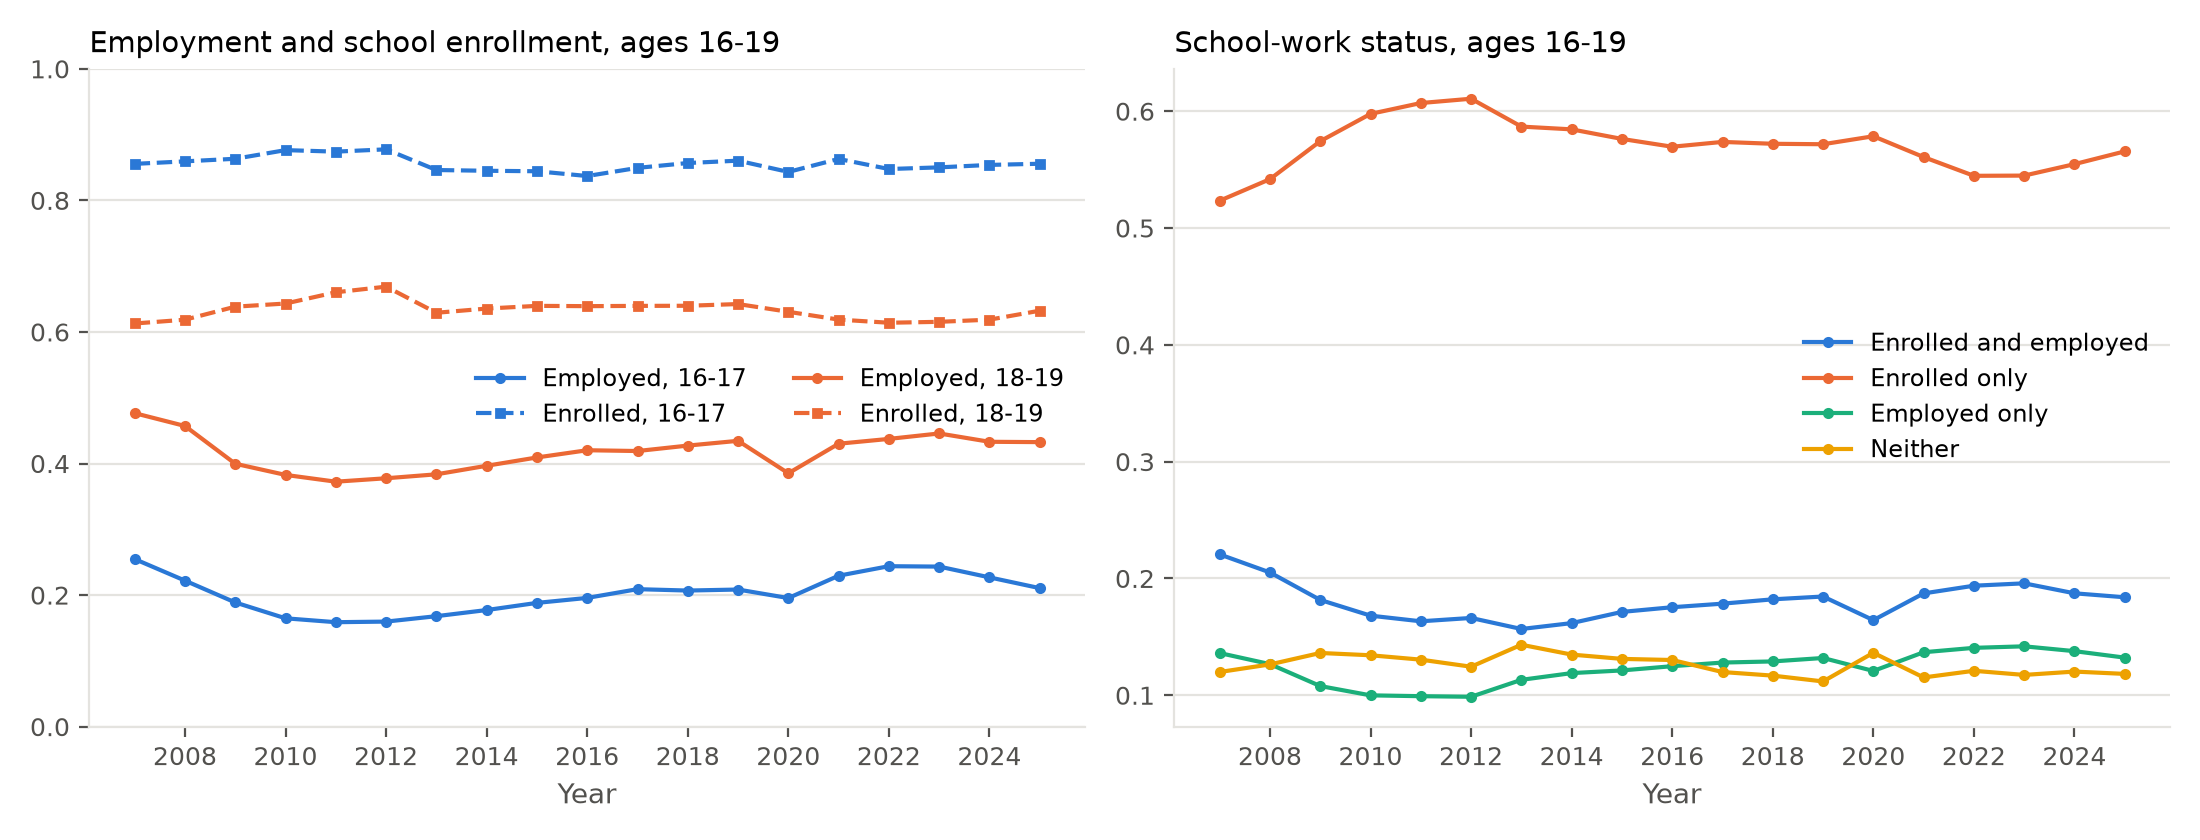
\includegraphics[width=\textwidth]{fig1_trends}
\caption{Employment, school enrollment and school--work status of 16--19 year olds, 1994--2025}
\label{fig:trends}
\begin{minipage}{\textwidth}\footnotesize Annual weighted means from the CPS basic monthly files, all months.\end{minipage}
\end{figure}

\begin{figure}[H]
\centering
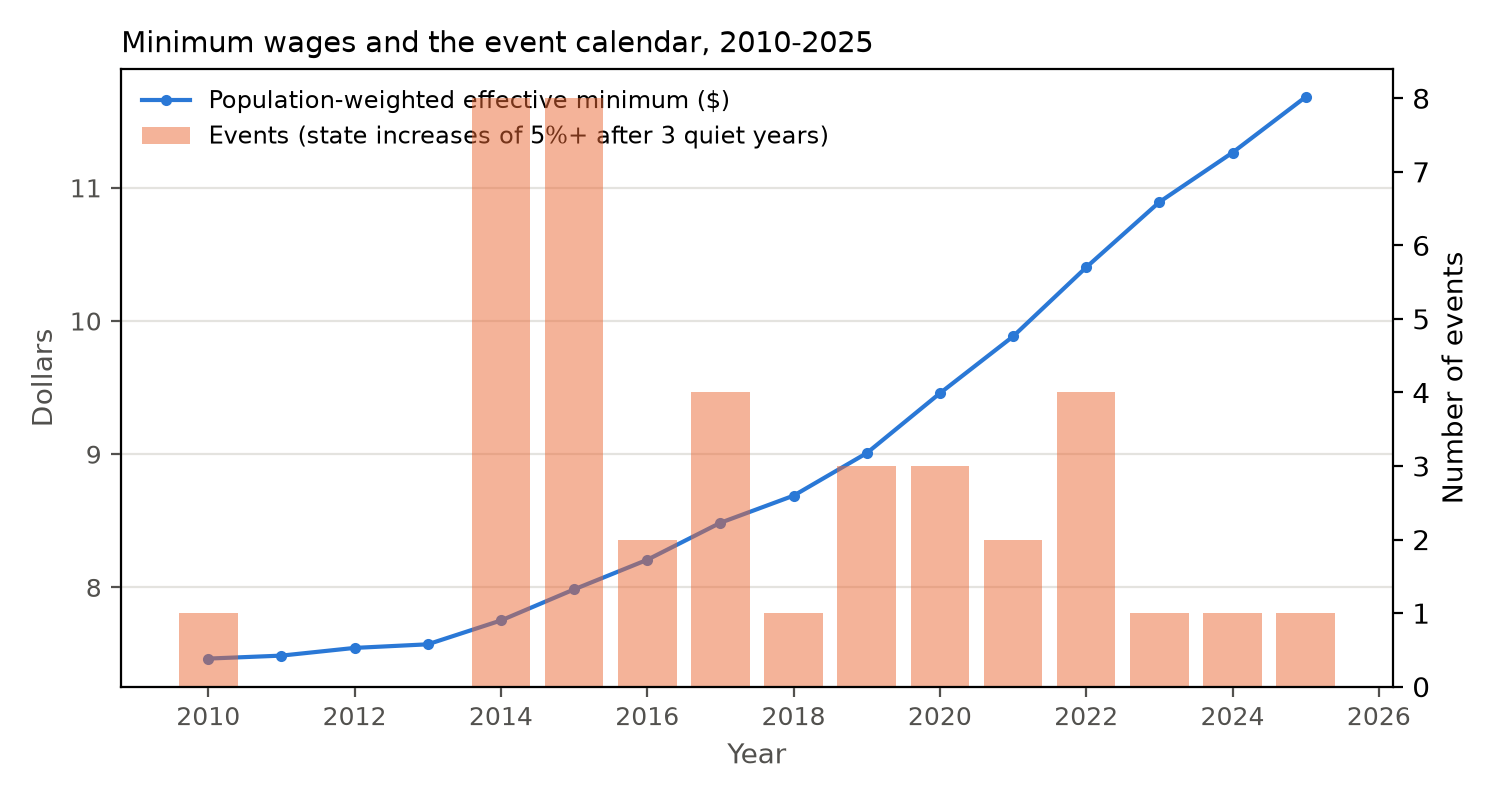
\includegraphics[width=0.85\textwidth]{fig2_minwage}
\caption{The effective minimum wage and the calendar of state events, 1994--2025}
\label{fig:minwage}
\begin{minipage}{\textwidth}\footnotesize Line: mean of the larger of the state and federal minimum, weighted by the state's teen population. Bars: number of state-driven increases of at least 5 percent after 36 months without one.\end{minipage}
\end{figure}

\section{Results}\label{sec:results}

\subsection{The events raised teen pay}

Figure~\ref{fig:firststage} and the first two rows of Table~\ref{tab:main} give the first stage. Among hourly-paid teens in the outgoing rotation groups, the hourly wage in the event units rises relative to controls by 1.8 percent in the year of the increase, 6.8 percent in the first full year after it, 5.5 percent in the second and 7.0 percent in the third for 16--17 year olds, and by 0.7, 3.6, 2.8 and 5.0 percent for 18--19 year olds; pooling the ages, by 0.9, 4.6, 3.6 and 6.0 percent. The post-event averages are 5.3 percent (s.e.\ 1.2), 3.0 percent (s.e.\ 0.9) and 3.8 percent (s.e.\ 0.9). The year-0 effect is small because that year averages up to eleven pre-increase months with the first months after, and because most schedules add their later steps in years 1 to 3; from year 1 the wage effect is five to seven standard errors from zero and grows with the schedule. The pre-event coefficients are within about one standard error of zero at both ages, with one $-2$ percent point at year $-3$ for the younger group that is not followed by anything at year $-2$. Weekly earnings of all teen workers, which combine the wage with hours, rise by 6 to 10 percent from year 1 at 16--17 and by 4 to 6 percent at 18--19.

The wage gain is about a seventh of the rise in the minimum. That is what one expects: a large share of hourly-paid teens already earn above the old minimum, the minimum binds most for the youngest and least experienced, and the ORG hourly wage question is asked only of those paid by the hour. The important point for what follows is that the events moved the pay of teenagers by an amount that is large relative to the precision of the outcome estimates, so a null on enrollment or employment is not a null on the treatment.

\begin{figure}[H]
\centering
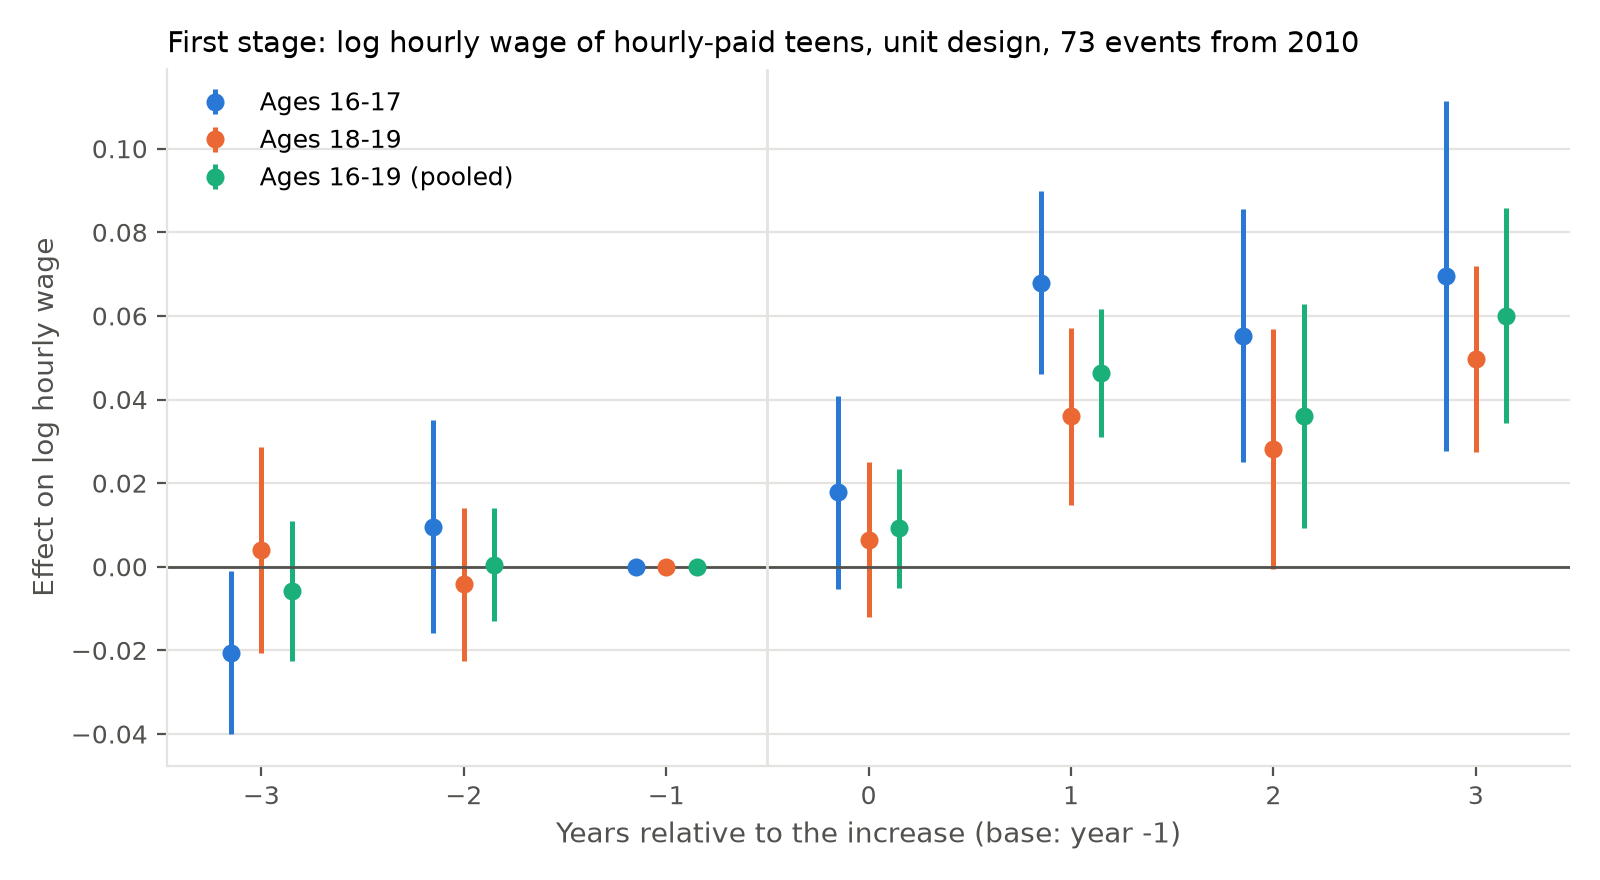
\includegraphics[width=0.9\textwidth]{fig3_first_stage}
\caption{First stage: log hourly wage of hourly-paid teens around the 73 events from 2010}
\label{fig:firststage}
\begin{minipage}{\textwidth}\footnotesize Effects relative to the year before the increase, population-weighted across events, for ages 16--17, 18--19 and 16--19 pooled; 95 percent intervals from the state block bootstrap.\end{minipage}
\end{figure}

\subsection{Enrollment, employment and the allocation of time did not change}

Table~\ref{tab:main} reports the post-event average effect on every outcome, by age, with the average of the pre-event coefficients beside it. Enrollment changes by $-0.3$ points (s.e.\ 0.4) at 16--17, $+0.1$ (s.e.\ 0.9) at 18--19 and $+0.1$ (s.e.\ 0.5) pooled; the 95 percent intervals exclude a decline larger than 1.1 points at the younger ages and 1.6 at the older. High school enrollment and full-time enrollment give the same answer. Employment changes by $-0.1$ points (s.e.\ 0.5) at 16--17 and $+1.0$ (s.e.\ 0.7) at 18--19, labour force participation by $+0.3$ (s.e.\ 0.5) and $+0.7$ (s.e.\ 0.5), and usual hours by $-0.04$ (s.e.\ 0.12) and $+0.30$ (s.e.\ 0.27). None of the four school--work states moves: enrolled-and-employed by $-0.3$ and $+0.7$ points, enrolled-only by $-0.0$ and $-0.5$, employed-only by $+0.2$ and $+0.3$, neither by $+0.1$ and $-0.5$, all with standard errors of 0.3 to 0.7 points. The pre-event averages are of the same order as the post-event ones and of no consistent sign.

\begin{table}[H]
\centering
\caption{Effects of minimum wage increases on teen outcomes: post-event average, 73 events from 2010}
\label{tab:main}
\small
\begin{tabular}{lcccccc}
\toprule
 & \multicolumn{2}{c}{Ages 16--17} & \multicolumn{2}{c}{Ages 18--19} & \multicolumn{2}{c}{Ages 16--19} \\
\cmidrule(lr){2-3}\cmidrule(lr){4-5}\cmidrule(lr){6-7}
 & Post & Pre & Post & Pre & Post & Pre \\
\midrule
Log hourly wage, hourly paid (ORG) & 0.054$^{***}$ & -0.005 & 0.030$^{***}$ & -0.005 & 0.039$^{***}$ & -0.005 \\
 & (0.013) &  & (0.009) &  & (0.009) &  \\
Log weekly earnings (ORG) & 0.054$^{*}$ & -0.008 & 0.045$^{*}$ & -0.004 & 0.051$^{**}$ & -0.004 \\
 & (0.033) &  & (0.025) &  & (0.025) &  \\
Enrolled in school & -0.002 & -0.003 & 0.000 & 0.004 & 0.001 & 0.003 \\
 & (0.004) &  & (0.010) &  & (0.005) &  \\
Enrolled in high school & -0.004 & -0.003 & -0.014$^{**}$ & -0.014 & -0.006 & -0.002 \\
 & (0.005) &  & (0.007) &  & (0.006) &  \\
Enrolled full time & -0.001 & -0.002 & -0.001 & 0.000 & 0.000 & 0.002 \\
 & (0.005) &  & (0.009) &  & (0.005) &  \\
Employed & -0.002 & -0.005 & 0.012 & 0.003 & 0.003 & -0.004 \\
 & (0.005) &  & (0.007) &  & (0.004) &  \\
In labor force & 0.002 & -0.001 & 0.008 & 0.004 & 0.003 & -0.002 \\
 & (0.005) &  & (0.005) &  & (0.004) &  \\
Usual weekly hours & -0.04 & -0.08 & 0.38 & 0.17 & 0.11 & -0.05 \\
 & (0.13) &  & (0.29) &  & (0.16) &  \\
Enrolled and employed & -0.003 & -0.003 & 0.007 & 0.004 & 0.001 & -0.001 \\
 & (0.005) &  & (0.007) &  & (0.004) &  \\
Enrolled only & 0.002 & 0.001 & -0.007 & -0.000 & -0.001 & 0.004 \\
 & (0.006) &  & (0.006) &  & (0.003) &  \\
Employed only & 0.001 & -0.002 & 0.005 & -0.002 & 0.002 & -0.003 \\
 & (0.003) &  & (0.008) &  & (0.004) &  \\
Neither enrolled nor employed & 0.000 & 0.004 & -0.005 & -0.002 & -0.003 & 0.001 \\
 & (0.004) &  & (0.005) &  & (0.003) &  \\
\bottomrule
\end{tabular}

\begin{tablenotes}\footnotesize
\item Post: average of the relative-year effects for years 0--3 after the increase, relative to year $-1$, population-weighted across events; block-bootstrap standard errors over states in parentheses (99 draws). Pre: average of the relative-year effects for years $-3$ and $-2$. Wage and earnings outcomes use the outgoing rotation groups and earnings weights. $^{*}$, $^{**}$, $^{***}$: significant at 10, 5 and 1 percent.
\end{tablenotes}
\end{table}

Figure~\ref{fig:eventmain} plots the coefficients by relative year for the wage, enrollment, employment and three of the four school--work states, for each age bracket and the two pooled, and Table~\ref{tab:eventtime} lists the wage, enrollment and employment coefficients. The enrollment series at 16--17 runs $-0.0$, $-0.2$, 0, $-0.3$, $-0.4$, $-0.3$, $-0.2$ points from year $-3$ to year 3, with standard errors of 0.3 to 0.7; at 18--19 it runs $+0.7$, $+0.4$, 0, $+0.4$, $-0.2$, $+0.6$, $-0.3$ with standard errors of 0.8 to 1.3. There is no break at the event and no drift after it. Employment at 18--19 shows post-event points of $+1.2$, $+0.9$, $+0.2$ and $+1.7$ against pre-event points of $-0.2$ and $-0.3$; the post-event average is 1.4 standard errors from zero and positive, the sign the wage-setting model allows and the competitive model does not.

\begin{figure}[H]
\centering
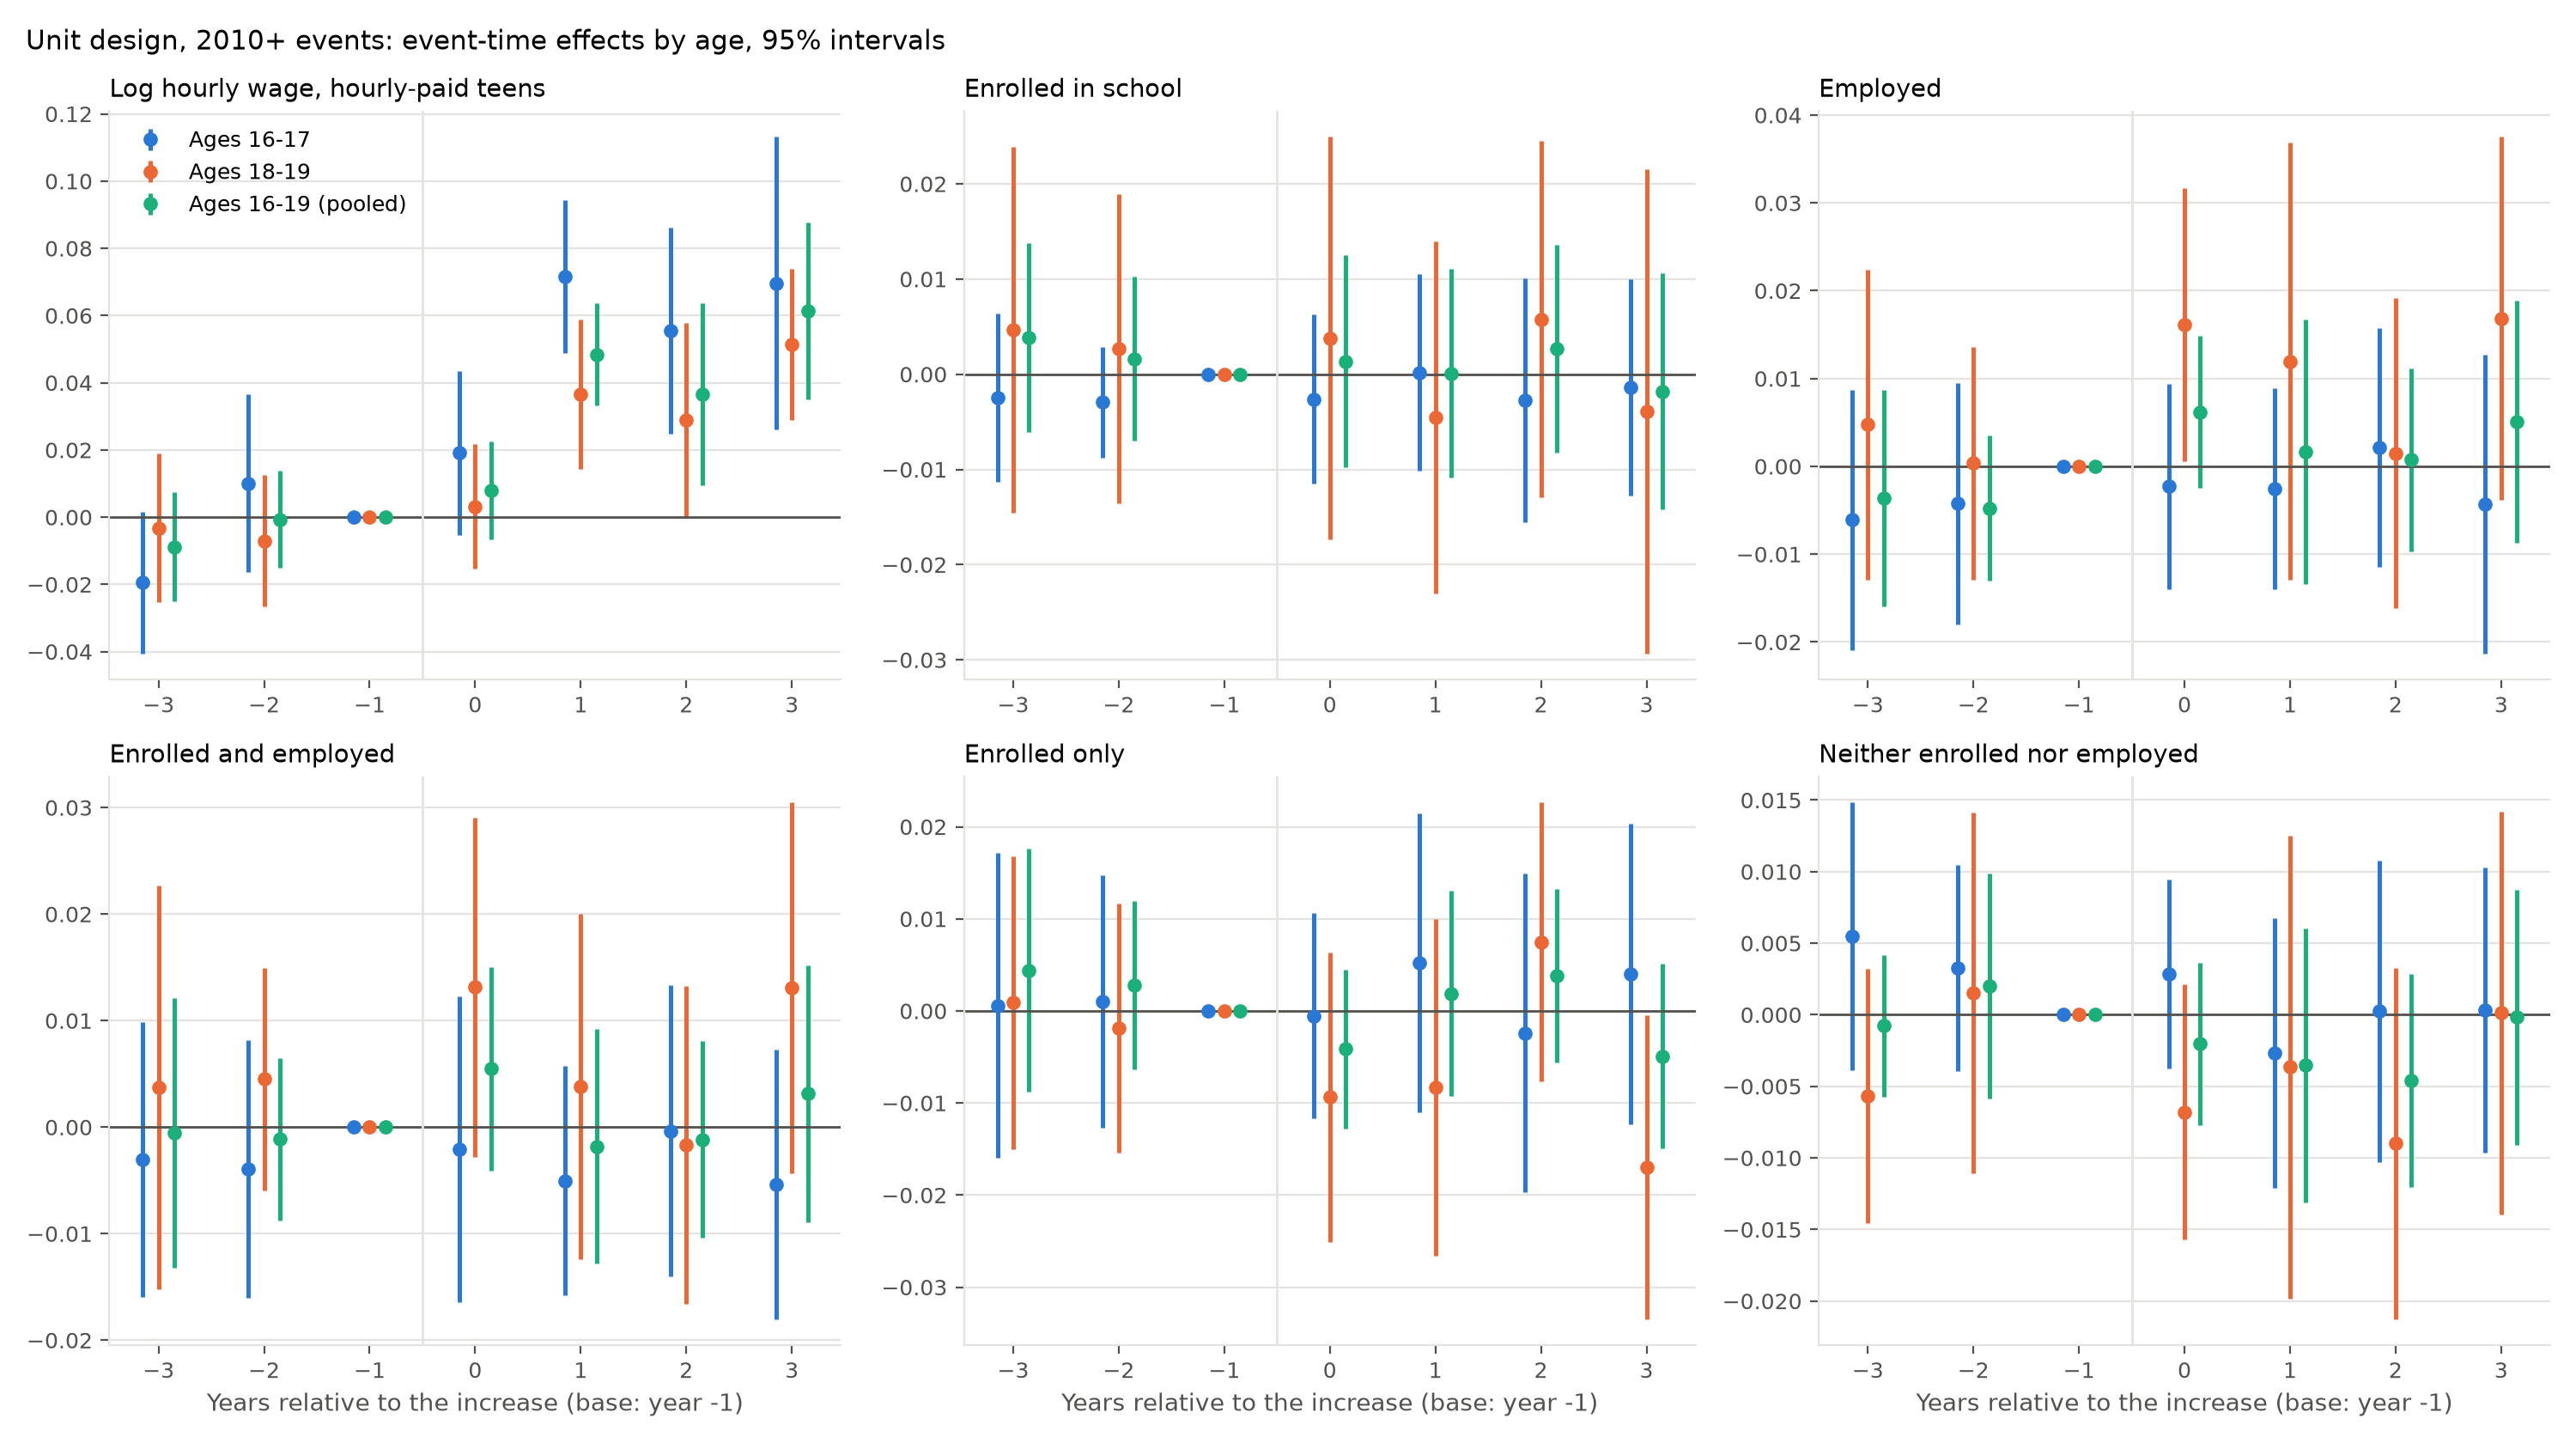
\includegraphics[width=\textwidth]{fig4_event_main}
\caption{Event-time effects on wages, enrollment, employment and school--work status, 73 events from 2010, by age}
\label{fig:eventmain}
\begin{minipage}{\textwidth}\footnotesize Effects relative to the year before the increase, population-weighted across events, for ages 16--17, 18--19 and 16--19 pooled; 95 percent intervals from the state block bootstrap. The employed-only state is omitted; it is the complement of the other three.\end{minipage}
\end{figure}

\begin{table}[H]
\centering
\caption{Event-time coefficients: log hourly wage, enrollment and employment, 73 events from 2010}
\label{tab:eventtime}
\small
\begin{tabular}{lcccccc}
\toprule
 & \multicolumn{2}{c}{Log hourly wage} & \multicolumn{2}{c}{Enrolled} & \multicolumn{2}{c}{Employed} \\
\cmidrule(lr){2-3}\cmidrule(lr){4-5}\cmidrule(lr){6-7}
 & 16--17 & 18--19 & 16--17 & 18--19 & 16--17 & 18--19 \\
\midrule
Year -3 & -0.019$^{*}$ & -0.003 & -0.002 & 0.005 & -0.006 & 0.005 \\
 & (0.011) & (0.011) & (0.005) & (0.010) & (0.008) & (0.009) \\
Year -2 & 0.010 & -0.007 & -0.003 & 0.003 & -0.004 & 0.000 \\
 & (0.013) & (0.010) & (0.003) & (0.008) & (0.007) & (0.007) \\
Year -1 & 0 & 0 & 0 & 0 & 0 & 0 \\
 &  &  &  &  &  &  \\
Year 0 & 0.019 & 0.003 & -0.003 & 0.004 & -0.002 & 0.016$^{**}$ \\
 & (0.012) & (0.009) & (0.005) & (0.011) & (0.006) & (0.008) \\
Year 1 & 0.072$^{***}$ & 0.037$^{***}$ & 0.000 & -0.005 & -0.003 & 0.012 \\
 & (0.012) & (0.011) & (0.005) & (0.009) & (0.006) & (0.013) \\
Year 2 & 0.056$^{***}$ & 0.029$^{*}$ & -0.003 & 0.006 & 0.002 & 0.002 \\
 & (0.016) & (0.015) & (0.007) & (0.010) & (0.007) & (0.009) \\
Year 3 & 0.070$^{***}$ & 0.051$^{***}$ & -0.001 & -0.004 & -0.004 & 0.017 \\
 & (0.022) & (0.011) & (0.006) & (0.013) & (0.009) & (0.011) \\
\bottomrule
\end{tabular}

\begin{tablenotes}\footnotesize
\item Relative year $-1$ is the twelve months before the increase and the omitted base. Block-bootstrap standard errors over states in parentheses.
\end{tablenotes}
\end{table}

Figure~\ref{fig:status} shows the four school--work states at 18--19 over the window. The enrolled-and-employed and employed-only shares drift up by half a point and the enrolled-only share down by half a point, with intervals of two to three points around each; nothing separates from zero. The shift from enrolled-and-employed to enrolled-only that \citet{neumark2019} attribute to the minimum wage would appear here as a fall in the blue series and a rise in the orange one. If anything the movements are in the opposite direction, and both are within noise.

\begin{figure}[H]
\centering
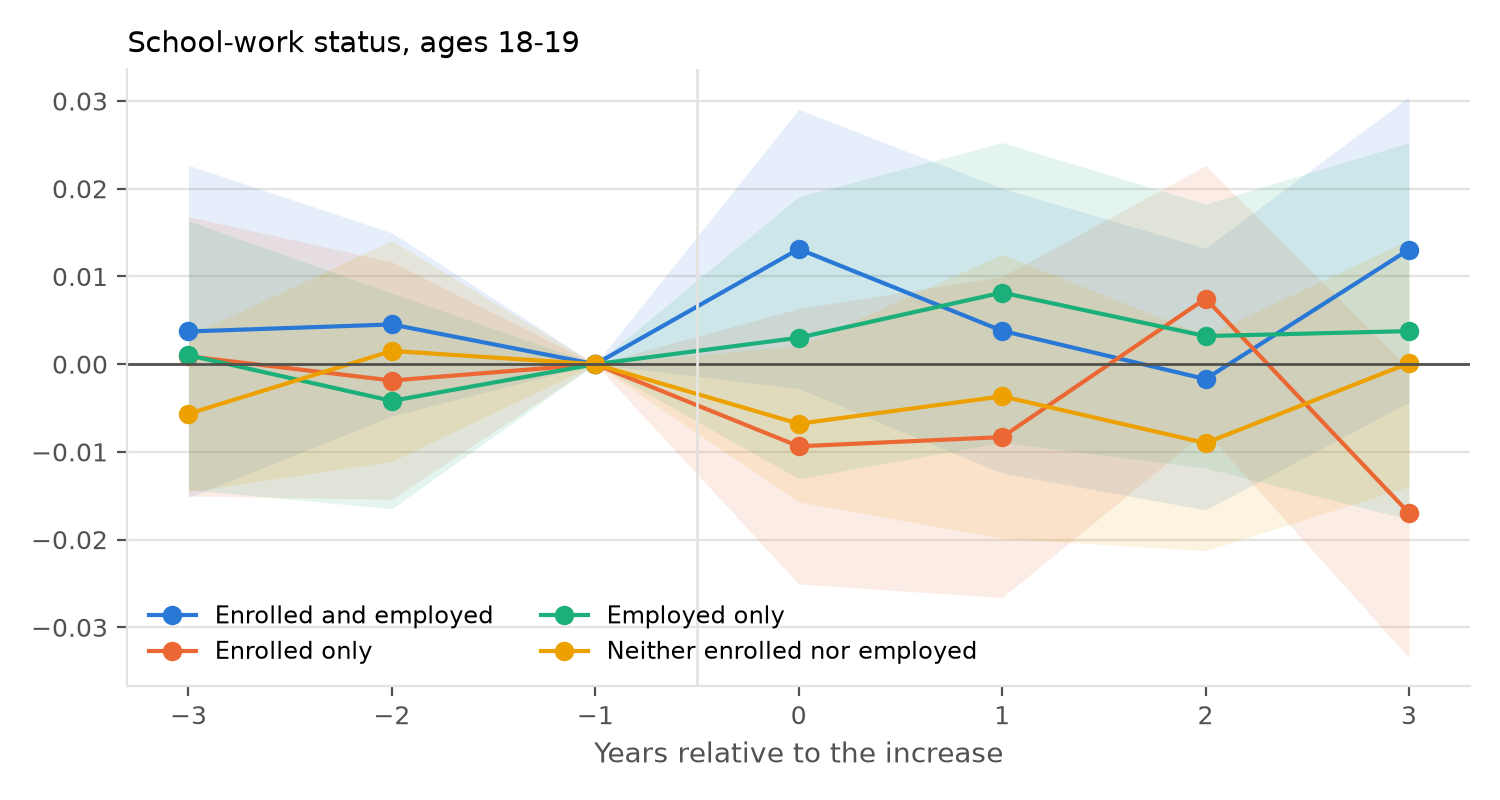
\includegraphics[width=0.85\textwidth]{fig5_status_1819}
\caption{School--work status of 18--19 year olds around the events}
\label{fig:status}
\begin{minipage}{\textwidth}\footnotesize Effects on the share in each of the four states, relative to the year before the increase; shaded bands are 95 percent intervals.\end{minipage}
\end{figure}

\subsection{Robustness}

Table~\ref{tab:robust} re-estimates the enrollment, employment and neither-enrolled-nor-employed effects under alternative units, event sets, control sets, weights and samples. Treating states as the units, so that a county's local minimum is ignored and its teens are counted at the state rate, gives enrollment effects of $-0.3$ (s.e.\ 0.4) and $-0.4$ (s.e.\ 0.9) from 39 state events, the same as the unit design; the state-level version of every figure and table is in Appendix~\ref{app:state}. Within the unit design, the 39 state-remainder events alone give $-0.5$ (0.5) and $-0.9$ (1.0). The 34 county events are discussed below. Using all 134 unit events since 1994 gives $-0.3$ (s.e.\ 0.3) and $+0.4$ (s.e.\ 0.6); the 61 events before 2010, whose windows contain the federal increases, give $-0.3$ and $+0.7$; the 62 events with a window rise of at least 20 percent give $-0.2$ and $-0.0$. Restricting controls to units with no increase of any kind or to the states at the federal floor, dropping 2020 and 2021, and using September to May only all leave the estimates within one standard error of zero. Equal weighting of events gives $+0.3$ (0.5) and $+1.8$ (0.9) at 18--19, the latter with a pre-event average of $+2.1$, because equal weights give the small county units, whose enrollment was already rising, the same weight as California. Employment of 16--17 year olds is $-1.0$ points (s.e.\ 0.7) in the pre-2010 set and $-0.5$ (0.4) across all events, the only estimates in the table that lean negative, and both are within two standard errors of zero and paired with zero enrollment effects. Ages 20--24, where the enrollment margin is college and the minimum binds less, show $-0.2$ (s.e.\ 0.7) on enrollment and $+0.1$ (s.e.\ 0.5) on employment.

\begin{table}[H]
\centering
\caption{Robustness: post-event averages under alternative units, event sets, controls, weights and samples}
\label{tab:robust}
\footnotesize
\begin{tabular}{lcccccccc}
\toprule
 & \multicolumn{2}{c}{Enrolled} & \multicolumn{2}{c}{Employed} & \multicolumn{2}{c}{Neither} & Events \\
\cmidrule(lr){2-3}\cmidrule(lr){4-5}\cmidrule(lr){6-7}
 & 16--17 & 18--19 & 16--17 & 18--19 & 16--17 & 18--19 & \\
\midrule
Main: unit design, 73 events from 2010, clean controls, population weights & -0.003 & 0.001 & -0.001 & 0.010 & 0.001 & -0.005 & 73 \\
 & (0.004) & (0.009) & (0.005) & (0.007) & (0.004) & (0.005) &  \\
State design (states as units), 39 events (Appendix) & -0.003 & -0.004 & -0.000 & 0.013 & 0.001 & -0.003 & 39 \\
 & (0.004) & (0.009) & (0.005) & (0.008) & (0.003) & (0.006) &  \\
Unit design: state-remainder events only (39) & -0.005 & -0.009 & 0.004 & 0.015$^{*}$ &  &  & 39 \\
 & (0.005) & (0.010) & (0.005) & (0.008) &  &  &  \\
Unit design: county events, state and local rise (18) & 0.005 & 0.033$^{***}$ & -0.021 & 0.003 &  &  & 18 \\
 & (0.007) & (0.009) & (0.029) & (0.023) &  &  &  \\
Unit design: county events, local rise only (16) & 0.016 & 0.075$^{**}$ & -0.016 & -0.047 &  &  & 16 \\
 & (0.017) & (0.034) & (0.028) & (0.051) &  &  &  \\
Large events only (window rise $\geq$ 20\%) & -0.002 & -0.000 & -0.002 & 0.014$^{*}$ & 0.001 & -0.005 & 62 \\
 & (0.004) & (0.010) & (0.005) & (0.007) & (0.004) & (0.005) &  \\
Strict controls (no rise of any kind) & -0.003 & 0.001 & -0.001 & 0.010 & 0.001 & -0.005 & 73 \\
 & (0.004) & (0.009) & (0.005) & (0.007) & (0.004) & (0.005) &  \\
Federal-floor controls only & -0.003 & -0.001 & -0.003 & 0.011 & 0.002 & -0.002 & 73 \\
 & (0.004) & (0.009) & (0.005) & (0.008) & (0.004) & (0.006) &  \\
Equal weight per event & 0.003 & 0.018$^{*}$ & -0.004 & -0.003 & -0.000 & -0.008 & 73 \\
 & (0.005) & (0.009) & (0.007) & (0.010) & (0.004) & (0.006) &  \\
Drop 2020--21 & -0.002 & 0.001 & -0.001 & 0.012 & -0.001 & -0.005 & 62 \\
 & (0.003) & (0.009) & (0.005) & (0.010) & (0.003) & (0.006) &  \\
September--May only & -0.006 & -0.002 & 0.001 & 0.011 & 0.004 & -0.003 & 73 \\
 & (0.004) & (0.007) & (0.006) & (0.008) & (0.002) & (0.006) &  \\
\bottomrule
\end{tabular}

\begin{tablenotes}\scriptsize
\item Each cell is the post-event average effect on the outcome for the age group; block-bootstrap standard errors in parentheses. Events: number of events in the specification.
\end{tablenotes}
\end{table}

The county events deserve a separate word. Their first stage is larger, 8.5 percent (s.e.\ 4.4) at 16--17 for the local-only events, because local increases were larger. Their enrollment estimates at 18--19 are positive: $+3.3$ points (s.e.\ 0.9) for the 18 county events with both a state and a local rise and $+7.5$ (3.4) for the 16 local-only events. Their pre-event averages are positive as well, $+1.3$ and $+5.3$: enrollment of 18--19 year olds in the big-city counties was rising relative to other states' units before the increases, which is what one expects of counties whose teenagers are increasingly the children of college-educated in-migrants. Net of the pre-event trend the post-event change is about two points in both sets, with the event counts and county samples of 13 to 40 teens a month that go with it. I read this as consistent with the main result and at most suggestive of a positive enrollment response where the increases were largest; it is not evidence that local minimums reduce enrollment, and the aggregate estimates, in which these events carry a fifth of the weight, are unaffected by them.

Figure~\ref{fig:byevent} shows the event-by-event enrollment estimates at 18--19. Thirty of the 73 are negative and 43 positive; the largest by weight, the California remainder in 2014, Florida in 2021 and Ohio in 2022, are $-1.9$, $+5.1$ and $0.0$ points, and Florida's pre-event average is the same $+5.2$, so its post-event figure is a level difference, not a response. No single event or unit drives the aggregate.

\begin{figure}[H]
\centering
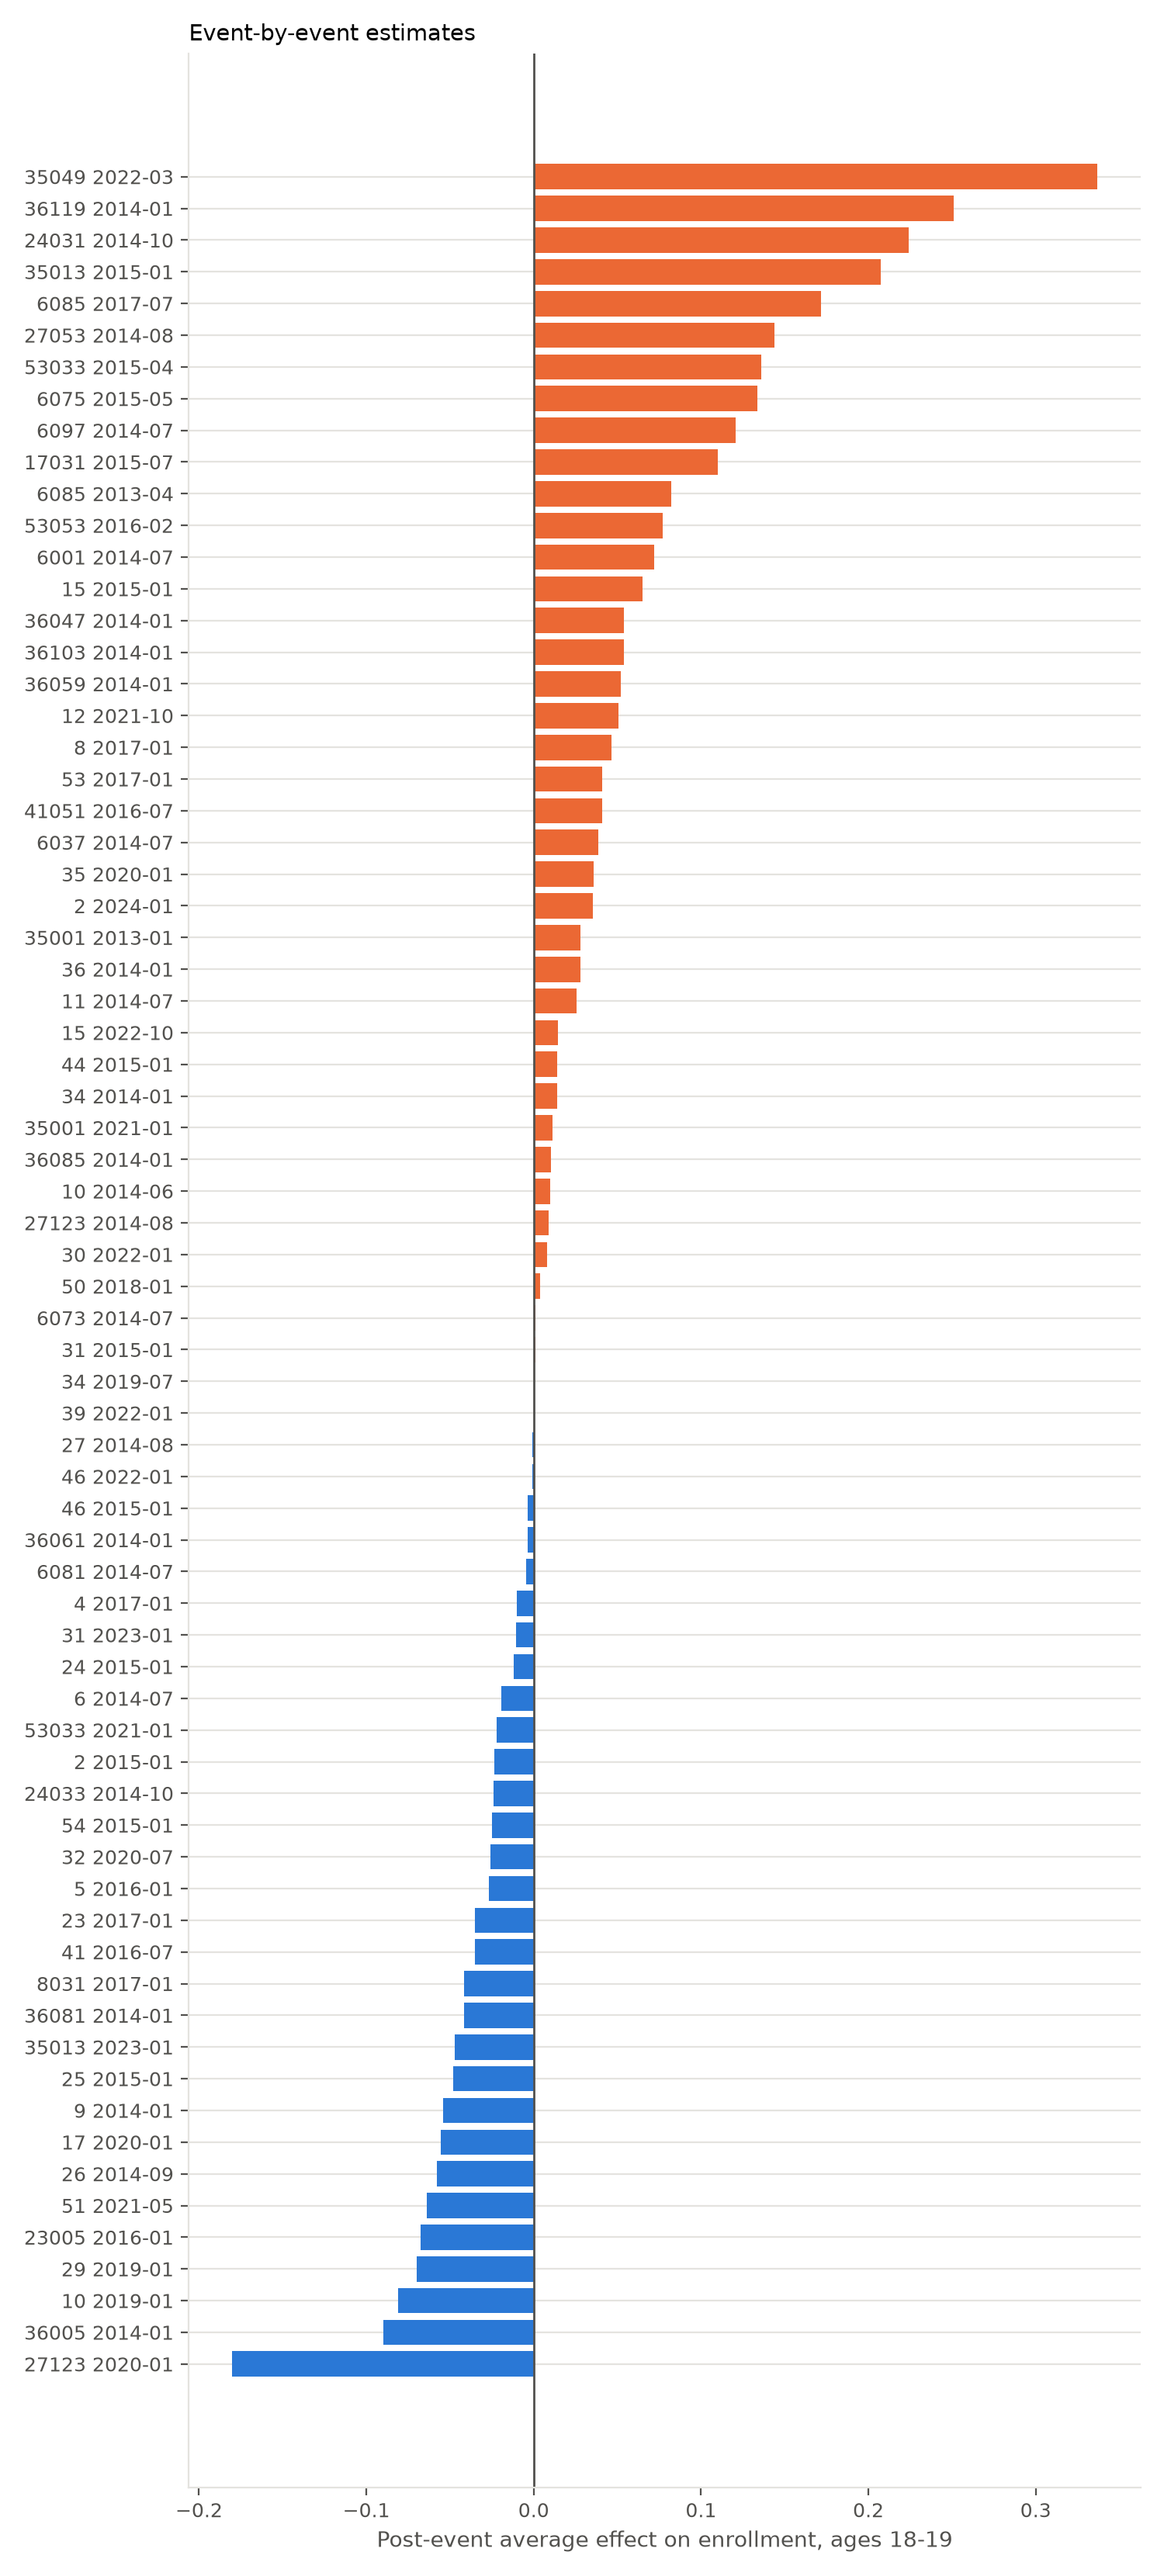
\includegraphics[width=0.85\textwidth]{fig6_byevent}
\caption{Event-by-event post-event averages, enrollment of 18--19 year olds}
\label{fig:byevent}
\begin{minipage}{\textwidth}\footnotesize Units are state FIPS codes (state remainders) and five-digit county codes (county units); the appendix table names them.\end{minipage}
\end{figure}

\subsection{Heterogeneity}

Table~\ref{tab:het} splits the enrollment estimate by sex, race and ethnicity, and family income. Every cell is within 1.5 points of zero except Black 18--19 year olds, at $+4.3$ (s.e.\ 2.9) with a pre-event average of $+1.7$, and none is within two standard errors of a negative effect. Boys aged 18--19, at $-1.1$ points (s.e.\ 1.0), have a pre-event average of $-2.0$, and girls, at $+1.3$ (1.1), one of $+3.2$; neither is evidence of a response. Teens in families below \$50,000, for whom the liquidity channel of Section~\ref{sec:theory} should matter most and the opportunity-cost channel bind hardest, show $-0.1$ (s.e.\ 0.8) at 16--17 and $+0.5$ (s.e.\ 1.5) at 18--19.

\begin{table}[H]
\centering
\caption{Heterogeneity in the enrollment effect, 73 events from 2010}
\label{tab:het}
\small
\begin{tabular}{lcccc}
\toprule
 & \multicolumn{2}{c}{Ages 16--17} & \multicolumn{2}{c}{Ages 18--19} \\
\cmidrule(lr){2-3}\cmidrule(lr){4-5}
 & Post & Pre & Post & Pre \\
\midrule
Girls & -0.000 & -0.001 & 0.012 & 0.030 \\
 & (0.005) &  & (0.012) &  \\
Boys & -0.002 & -0.004 & -0.011 & -0.024 \\
 & (0.005) &  & (0.011) &  \\
Black & -0.001 & -0.006 & 0.043 & 0.016 \\
 & (0.014) &  & (0.030) &  \\
Hispanic & -0.003 & -0.000 & -0.006 & -0.007 \\
 & (0.009) &  & (0.022) &  \\
White and other & 0.000 & 0.000 & -0.012 & 0.001 \\
 & (0.006) &  & (0.011) &  \\
\bottomrule
\end{tabular}

\begin{tablenotes}\footnotesize
\item Post: post-event average; Pre: average of years $-3$ and $-2$. Family income is the CPS household income category, split at \$50,000.
\end{tablenotes}
\end{table}

\section{The fall in teen employment}\label{sec:discussion}

The estimates rule the minimum wage out as the cause of the decline in teen employment on two counts of timing and one of magnitude. First, most of the decline happened between 2000 and 2010 (Figure~\ref{fig:trends}), before the large state and local schedules that give the minimum wage its modern bite; the events of 1994--2009 were smaller, and the estimates for them are zero on employment at 18--19 and $-1.0$ points (s.e.\ 0.7) at 16--17. Second, the period of the largest increases, 2014--2025, is one in which teen employment rose, from 28 to 33 percent. Third, the magnitude: even taking the most negative estimate in Table~\ref{tab:robust} at face value and applying it to every teen exposed to an event, the minimum wage would account for about one point of an eighteen-point decline.

What the estimates say instead is that the increases transferred income to teenagers who work. A 5 percent wage gain on annual earnings of \$8,000 to \$13,000, for the fifth of 16--17 year olds and two fifths of 18--19 year olds who are employed, with no loss of jobs, hours or schooling, is an unambiguous gain in the model of Section~\ref{sec:theory}, and one that the wage-setting case predicts and the competitive case does not. The finding is consistent with the bunching estimates of \citet{cengiz2019} for all low-wage workers and with the direct evidence of employer wage-setting power in the markets where teens work \citep{azar2019,manning2003}.

The decline itself then needs another explanation, and the candidates in \citet{neumark2019} and \citet{smith2011,smith2012} remain: the rising return to schooling and the intensification of college preparation, which raise the value of time spent on school rather than work; competition from adult and immigrant workers in the retail and food service jobs that teens held; and the two recessions of the period, whose effects on youth employment were large and slow to reverse. The enrollment series in Figure~\ref{fig:trends} rose steadily through 2012 and has been flat since, while employment has recovered, which fits a story in which the schooling margin moved for reasons unrelated to the wage floor and the labour market for teens then tightened. Distinguishing among those explanations requires designs suited to each; this paper's contribution is to remove one from the list.

Three limits should be stated. The enrollment measure is attendance last week; it cannot see grade progression, dropout timing or completion, so the null does not rule out effects on attainment measured years later, which administrative or ACS data would be needed to test. The 2023--2025 minimum wage changes and index adjustments are compiled from state sources and are less thoroughly vetted than the \citet{vaghul2016} list; they determine which units are clean controls after 2022 and should be verified before the event list is treated as final. Local minimums are carried at their end-2022 levels thereafter, and a city's rate is applied to its whole county, so a Seattle rate treats all of King County and a Portland rate all of Cumberland County; the county samples are small and the county events are best read alongside the state remainders rather than on their own. Standard errors are from a 99-draw block bootstrap; the wild cluster bootstrap in the Stata replication is the inference to report.

\section{Conclusion}\label{sec:conclusion}

Employment of American teenagers fell by eighteen points in the 2000s, and the most prominent explanation from panel regressions is that state minimum wages priced them out of work and into school. Using the event design that the minimum wage employment literature adopted after 2019, with every county that sets its own minimum treated as a jurisdiction of its own, 73 large increases since 2010 compared against clean controls in monthly CPS data on 16--19 year olds, I find that the increases raised the hourly wages of working teens by 3 to 7 percent and changed nothing else: not enrollment, not employment, not hours, not labour force participation, and not the division of teenagers among school, work, both and neither. The estimates are precise enough to rule out enrollment effects larger than a point or two and employment effects larger than a point at the ages the minimum binds most, and they are stable across units, event sets, control groups, weights, the pandemic years and subgroups. A two-period schooling model shows that this is the expected outcome when the wage gain is small relative to the skilled premium and employers have wage-setting power: the minimum wage raises pay without reducing the probability of a job, and a few hundred dollars a year does not move a decision worth several hundred thousand. The minimum wage is not the culprit in the fall of teen employment. Over this period it functioned as a transfer to teenagers who work, with no offsetting cost in their schooling or their jobs.

\clearpage
\bibliographystyle{aer}
\begin{thebibliography}{99}

\bibitem[Acemoglu(2009)]{acemoglu_notes} Acemoglu, Daron. 2009. Lectures in Labor Economics. Lecture notes, Massachusetts Institute of Technology.

\bibitem[Allegretto et al.(2017)]{allegretto2017} Allegretto, Sylvia, Arindrajit Dube, Michael Reich, and Ben Zipperer. 2017. ``Credible Research Designs for Minimum Wage Studies: A Response to Neumark, Salas, and Wascher.'' \textit{ILR Review} 70 (3): 559--592.

\bibitem[Azar et al.(2019)]{azar2019} Azar, Jos\'e, Emiliano Huet-Vaughn, Ioana Marinescu, Bledi Taska, and Till von Wachter. 2019. ``Minimum Wage Employment Effects and Labor Market Concentration.'' NBER Working Paper 26101.

\bibitem[Baker et al.(2022)]{baker2022} Baker, Andrew C., David F. Larcker, and Charles C. Y. Wang. 2022. ``How Much Should We Trust Staggered Difference-in-Differences Estimates?'' \textit{Journal of Financial Economics} 144 (2): 370--395.

\bibitem[Callaway and Sant'Anna(2021)]{callaway2021} Callaway, Brantly, and Pedro H. C. Sant'Anna. 2021. ``Difference-in-Differences with Multiple Time Periods.'' \textit{Journal of Econometrics} 225 (2): 200--230.

\bibitem[Campolieti et al.(2005)]{campolieti2005} Campolieti, Michele, Tony Fang, and Morley Gunderson. 2005. ``How Minimum Wages Affect Schooling-Employment Outcomes in Canada, 1993--1999.'' \textit{Journal of Labor Research} 26 (3): 533--545.

\bibitem[Card and Krueger(1994)]{card1994} Card, David, and Alan B. Krueger. 1994. ``Minimum Wages and Employment: A Case Study of the Fast-Food Industry in New Jersey and Pennsylvania.'' \textit{American Economic Review} 84 (4): 772--793.

\bibitem[Cengiz et al.(2019)]{cengiz2019} Cengiz, Doruk, Arindrajit Dube, Attila Lindner, and Ben Zipperer. 2019. ``The Effect of Minimum Wages on Low-Wage Jobs.'' \textit{Quarterly Journal of Economics} 134 (3): 1405--1454.

\bibitem[Chaplin et al.(2003)]{chaplin2003} Chaplin, Duncan D., Mark D. Turner, and Andreas D. Pape. 2003. ``Minimum Wages and School Enrollment of Teenagers: A Look at the 1990's.'' \textit{Economics of Education Review} 22 (1): 11--21.

\bibitem[Clemens and Wither(2019)]{clemens2019} Clemens, Jeffrey, and Michael Wither. 2019. ``The Minimum Wage and the Great Recession: Evidence of Effects on the Employment and Income Trajectories of Low-Skilled Workers.'' \textit{Journal of Public Economics} 170: 53--67.

\bibitem[de Chaisemartin and D'Haultf{\oe}uille(2020)]{dechaisemartin2020} de Chaisemartin, Cl\'ement, and Xavier D'Haultf{\oe}uille. 2020. ``Two-Way Fixed Effects Estimators with Heterogeneous Treatment Effects.'' \textit{American Economic Review} 110 (9): 2964--2996.

\bibitem[de Chaisemartin and D'Haultf{\oe}uille(2024)]{dechaisemartin2024} de Chaisemartin, Cl\'ement, and Xavier D'Haultf{\oe}uille. 2024. ``Difference-in-Differences Estimators of Intertemporal Treatment Effects.'' \textit{Review of Economics and Statistics}, forthcoming.

\bibitem[Dube et al.(2010)]{dube2010} Dube, Arindrajit, T. William Lester, and Michael Reich. 2010. ``Minimum Wage Effects Across State Borders: Estimates Using Contiguous Counties.'' \textit{Review of Economics and Statistics} 92 (4): 945--964.

\bibitem[Dube(2019)]{dube2019} Dube, Arindrajit. 2019. ``Impacts of Minimum Wages: Review of the International Evidence.'' Report to the UK Low Pay Commission, HM Treasury.

\bibitem[Ehrenberg and Marcus(1982)]{ehrenberg1982} Ehrenberg, Ronald G., and Alan J. Marcus. 1982. ``Minimum Wages and Teenagers' Enrollment-Employment Outcomes: A Multinomial Logit Model.'' \textit{Journal of Human Resources} 17 (1): 39--58.

\bibitem[Flood et al.(2024)]{ipumscps} Flood, Sarah, Miriam King, Renae Rodgers, Steven Ruggles, J. Robert Warren, Daniel Backman, Annie Chen, Grace Cooper, Stephanie Richards, Megan Schouweiler, and Michael Westberry. 2024. \textit{IPUMS CPS: Version 12.0}. Minneapolis, MN: IPUMS.

\bibitem[Goodman-Bacon(2021)]{goodmanbacon2021} Goodman-Bacon, Andrew. 2021. ``Difference-in-Differences with Variation in Treatment Timing.'' \textit{Journal of Econometrics} 225 (2): 254--277.

\bibitem[Manning(2003)]{manning2003} Manning, Alan. 2003. \textit{Monopsony in Motion: Imperfect Competition in Labor Markets}. Princeton: Princeton University Press.

\bibitem[Mincer(1976)]{mincer1976} Mincer, Jacob. 1976. ``Unemployment Effects of Minimum Wages.'' \textit{Journal of Political Economy} 84 (4): S87--S104.

\bibitem[Morisi(2008)]{morisi2008} Morisi, Teresa L. 2008. ``Youth Enrollment and Employment during the School Year.'' \textit{Monthly Labor Review} 131 (2): 51--63.

\bibitem[Neumark and Shupe(2019)]{neumark2019} Neumark, David, and Cortnie Shupe. 2019. ``Declining Teen Employment: Minimum Wages, Returns to Schooling, and Immigration.'' \textit{Labour Economics} 59: 49--68.

\bibitem[Neumark and Wascher(1995a)]{neumark1995a} Neumark, David, and William Wascher. 1995a. ``Minimum Wage Effects on Employment and School Enrollment.'' \textit{Journal of Business and Economic Statistics} 13 (2): 199--206.

\bibitem[Neumark and Wascher(1995b)]{neumark1995b} Neumark, David, and William Wascher. 1995b. ``Minimum-Wage Effects on School and Work Transitions of Teenagers.'' \textit{American Economic Review} 85 (2): 244--249.

\bibitem[Neumark and Wascher(2003)]{neumark2003} Neumark, David, and William Wascher. 2003. ``Minimum Wages and Skill Acquisition: Another Look at Schooling Effects.'' \textit{Economics of Education Review} 22 (1): 1--10.

\bibitem[Smith(2011)]{smith2011} Smith, Christopher L. 2011. ``Polarization, Immigration, Education: What's Behind the Dramatic Decline in Youth Employment?'' Finance and Economics Discussion Series 2011-41, Federal Reserve Board.

\bibitem[Smith(2012)]{smith2012} Smith, Christopher L. 2012. ``The Impact of Low-Skilled Immigration on the Youth Labor Market.'' \textit{Journal of Labor Economics} 30 (1): 55--89.

\bibitem[Stigler(1946)]{stigler1946} Stigler, George J. 1946. ``The Economics of Minimum Wage Legislation.'' \textit{American Economic Review} 36 (3): 358--365.

\bibitem[Sun and Abraham(2021)]{sun2021} Sun, Liyang, and Sarah Abraham. 2021. ``Estimating Dynamic Treatment Effects in Event Studies with Heterogeneous Treatment Effects.'' \textit{Journal of Econometrics} 225 (2): 175--199.

\bibitem[Vaghul and Zipperer(2016)]{vaghul2016} Vaghul, Kavya, and Ben Zipperer. 2016. ``Historical State and Sub-State Minimum Wage Data.'' Washington Center for Equitable Growth Working Paper.

\bibitem[Warren and Hamrock(2010)]{warren2010} Warren, John Robert, and Caitlin Hamrock. 2010. ``The Effect of Minimum Wage Rates on High School Completion.'' \textit{Social Forces} 88 (3): 1379--1392.

\end{thebibliography}

\clearpage
\appendix
\section{The events}

\begin{table}[H]
\centering
\caption{Unit events from January 2010 with CPS teens in the unit}
\label{tab:events}
\scriptsize
\begin{tabular}{llrrrrrr}
\toprule
State & Event month & Before & First step & End of window & Rise (\%) & Steps & Controls \\
\midrule
Alaska & 2010-01 & 7.25 & 7.75 & 7.75 & 7 & 1 & 24 \\
New York & 2014-01 & 7.25 & 8.00 & 9.70 & 34 & 3 & 29 \\
New Jersey & 2014-01 & 7.25 & 8.25 & 8.44 & 16 & 1 & 29 \\
Connecticut & 2014-01 & 8.25 & 8.70 & 10.10 & 22 & 3 & 29 \\
Delaware & 2014-06 & 7.25 & 7.75 & 8.25 & 14 & 2 & 28 \\
California & 2014-07 & 8.00 & 9.00 & 11.00 & 38 & 3 & 28 \\
District of Columbia & 2014-07 & 8.25 & 9.50 & 12.50 & 52 & 4 & 28 \\
Minnesota & 2014-08 & 7.25 & 8.00 & 9.65 & 33 & 3 & 28 \\
Michigan & 2014-09 & 7.40 & 8.15 & 9.25 & 25 & 1 & 28 \\
South Dakota & 2015-01 & 7.25 & 8.50 & 8.85 & 22 & 1 & 28 \\
Rhode Island & 2015-01 & 8.00 & 9.00 & 10.10 & 26 & 3 & 28 \\
Nebraska & 2015-01 & 7.25 & 8.00 & 9.00 & 24 & 2 & 28 \\
Massachusetts & 2015-01 & 8.00 & 9.00 & 11.00 & 38 & 3 & 28 \\
Maryland & 2015-01 & 7.25 & 8.00 & 10.10 & 39 & 4 & 28 \\
West Virginia & 2015-01 & 7.25 & 8.00 & 8.75 & 21 & 2 & 28 \\
Alaska & 2015-01 & 7.75 & 8.75 & 9.84 & 27 & 2 & 28 \\
Hawaii & 2015-01 & 7.25 & 7.75 & 10.10 & 39 & 4 & 28 \\
Arkansas & 2016-01 & 7.50 & 8.00 & 9.25 & 23 & 3 & 27 \\
Oregon & 2016-07 & 9.25 & 9.75 & 11.25 & 22 & 2 & 25 \\
Arizona & 2017-01 & 8.05 & 10.00 & 12.00 & 49 & 3 & 24 \\
Colorado & 2017-01 & 8.31 & 9.30 & 12.00 & 44 & 4 & 24 \\
Maine & 2017-01 & 7.50 & 9.00 & 12.00 & 60 & 4 & 24 \\
Washington & 2017-01 & 9.47 & 11.00 & 13.50 & 43 & 2 & 24 \\
Vermont & 2018-01 & 10.00 & 10.50 & 11.75 & 18 & 2 & 23 \\
Delaware & 2019-01 & 8.25 & 8.75 & 10.50 & 27 & 3 & 21 \\
Missouri & 2019-01 & 7.85 & 8.60 & 11.15 & 42 & 4 & 21 \\
New Jersey & 2019-07 & 8.85 & 10.00 & 14.00 & 58 & 5 & 23 \\
Illinois & 2020-01 & 8.25 & 9.25 & 13.00 & 58 & 5 & 24 \\
New Mexico & 2020-01 & 7.50 & 9.00 & 12.00 & 60 & 3 & 24 \\
Nevada & 2020-07 & 8.25 & 9.00 & 11.25 & 36 & 4 & 23 \\
Virginia & 2021-05 & 7.25 & 9.50 & 13.50 & 86 & 4 & 22 \\
Florida & 2021-10 & 8.56 & 10.00 & 13.00 & 52 & 4 & 22 \\
Montana & 2022-01 & 8.75 & 9.20 & 10.55 & 21 & 2 & 22 \\
South Dakota & 2022-01 & 9.45 & 9.95 & 11.50 & 22 & 2 & 22 \\
Ohio & 2022-01 & 8.80 & 9.30 & 10.70 & 22 & 2 & 22 \\
Hawaii & 2022-10 & 10.10 & 12.00 & 14.00 & 39 & 2 & 22 \\
Nebraska & 2023-01 & 9.00 & 10.50 & 13.50 & 50 & 3 & 22 \\
Alaska & 2024-01 & 10.85 & 11.73 & 13.00 & 20 & 2 & 22 \\
Michigan & 2025-03 & 10.56 & 12.48 & 12.48 & 18 & 1 & 25 \\
\bottomrule
\end{tabular}

\begin{tablenotes}\scriptsize
\item Units: state remainders (the state outside its counties with a local minimum) and counties with their own minimum. Source: whether the rise came from the state rate, the local rate, or both in the same month. Before: effective minimum in the month before the event. First step: minimum in the event month. End of window: minimum 47 months after the event. Rise: end of window relative to before. Steps: number of increases of 5 percent or more in the window. Controls: units in other states with no increase of 5 percent or more from 36 months before to 47 months after the event. County rates are the county-wide rate where one exists and otherwise the largest city's, applied to the whole county. Alaska 2024 and Michigan 2025 rest on the post-2022 additions to the change list. Source: \citet{vaghul2016}, extended by the author.
\end{tablenotes}
\end{table}

\clearpage
\section{The state design}\label{app:state}

The state design ignores local minimums: each state is one unit at the state rate, and events are the 39 state increases from 2010 that satisfy the same rule. Its post-event averages are the second row of each block in Table~\ref{tab:robust}; Figures~\ref{fig:statewage} and \ref{fig:stateevent} are the state-design counterparts of Figures~\ref{fig:firststage} and \ref{fig:eventmain}. The wage first stage is 5.1 percent (s.e.\ 1.2) at 16--17 and 3.1 (0.9) at 18--19; enrollment $-0.3$ (0.4) and $-0.4$ (0.9); employment $0.0$ (0.5) and $+1.3$ (0.8).

\begin{figure}[H]
\centering
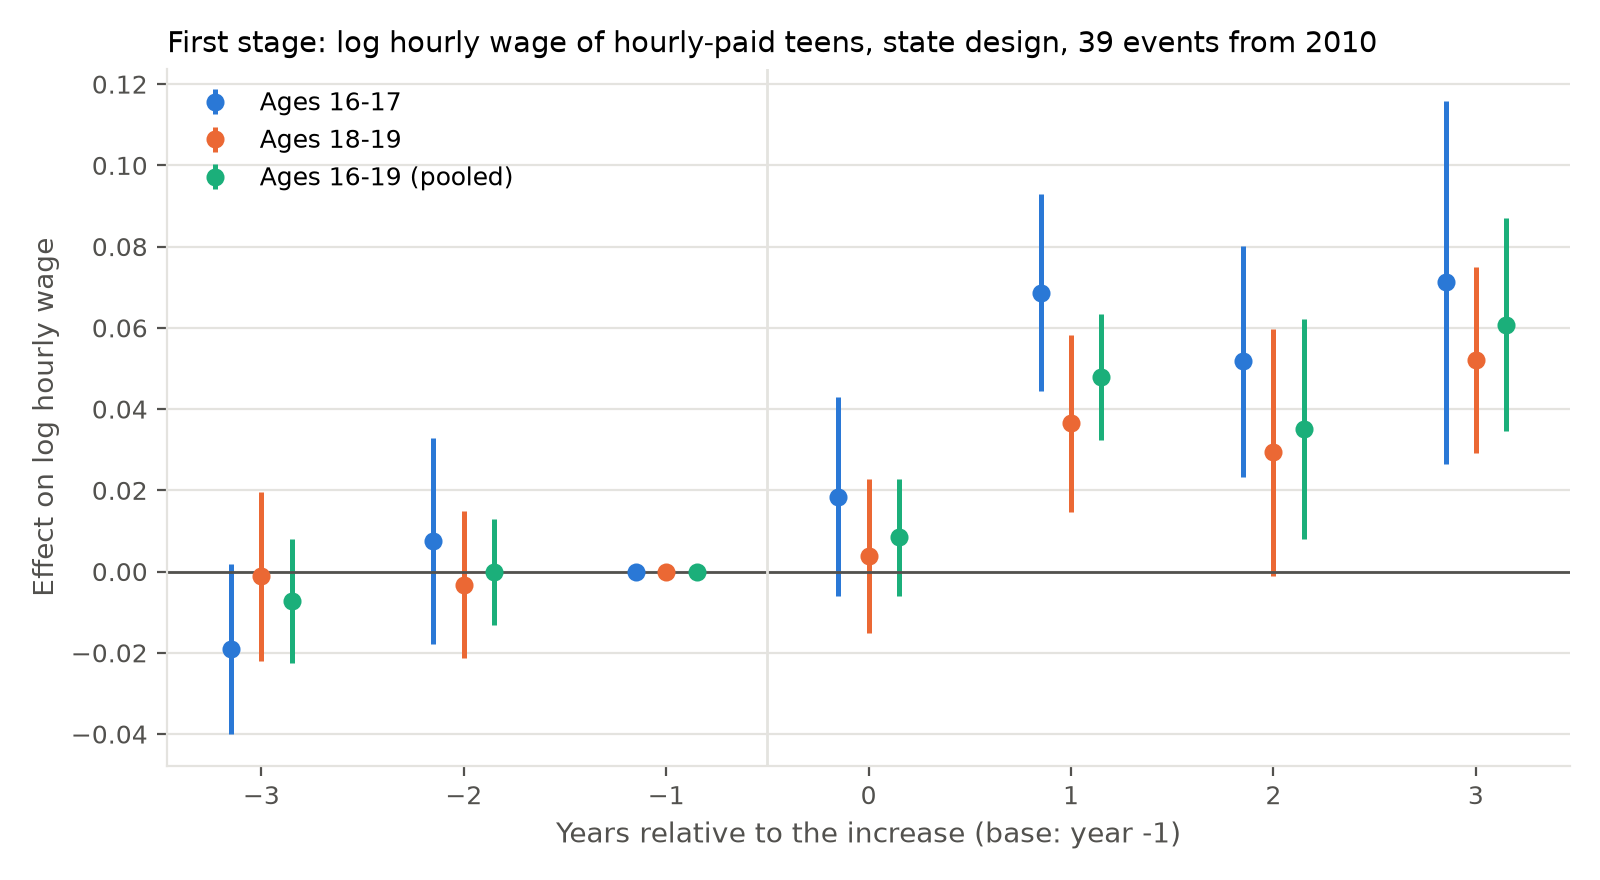
\includegraphics[width=0.9\textwidth]{figA1_state_first_stage}
\caption{State design: first stage, 39 state events from 2010}
\label{fig:statewage}
\end{figure}

\begin{figure}[H]
\centering
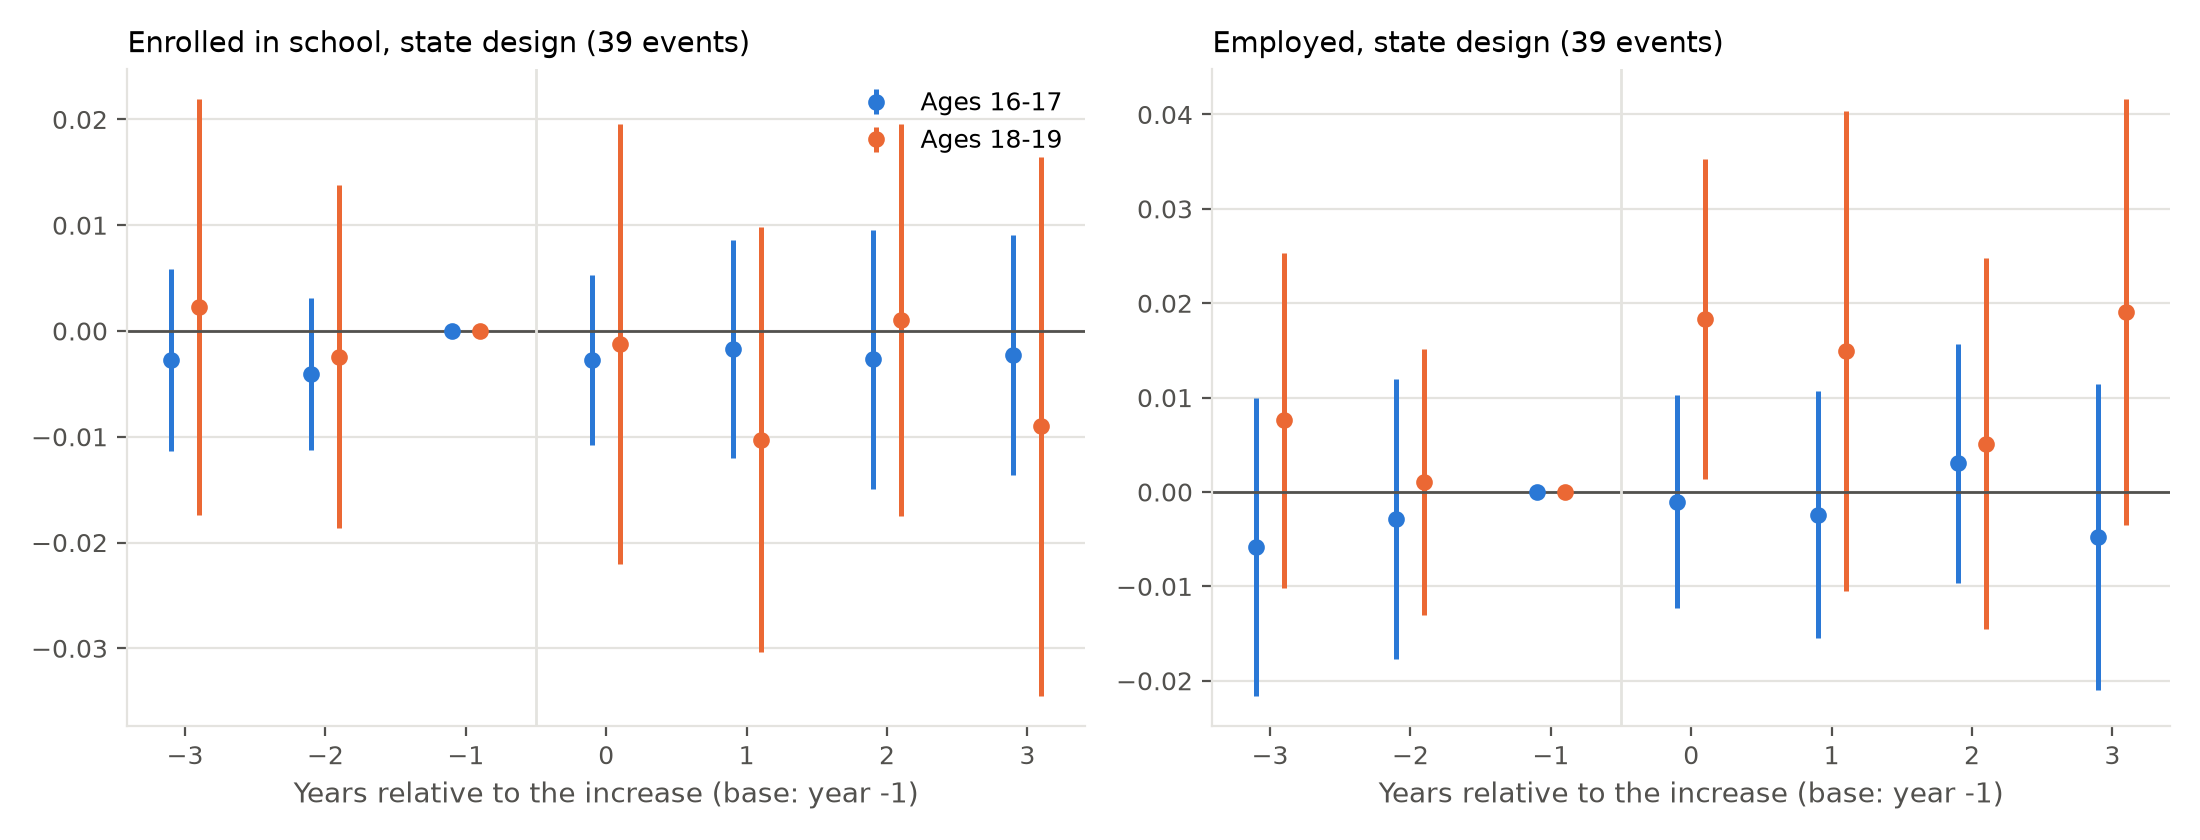
\includegraphics[width=\textwidth]{figA2_state_event_main}
\caption{State design: enrollment and employment, 39 state events from 2010}
\label{fig:stateevent}
\end{figure}

\end{document}
